\documentclass{article}

% if you need to pass options to natbib, use, e.g.:
% \PassOptionsToPackage{numbers, compress}{natbib}
% before loading nips_2017
%
% to avoid loading the natbib package, add option nonatbib:
\usepackage{nips_2017}


% to compile a camera-ready version, add the [final] option, e.g.:
% \usepackage[final]{nips_2017}

\usepackage[utf8]{inputenc} % allow utf-8 input
\usepackage[T1]{fontenc}    % use 8-bit T1 fonts
\usepackage{hyperref}       % hyperlinks
\usepackage{url}            % simple URL typesetting
\usepackage{booktabs}       % professional-quality tables
\usepackage{amsfonts}       % blackboard math symbols
\usepackage{nicefrac}       % compact symbols for 1/2, etc.
\usepackage{microtype}      % microtypography
\usepackage{natbib}
\usepackage[mathscr]{euscript}
\RequirePackage{amsthm,amsmath}
\usepackage{algorithm,algpseudocode}
\usepackage{color}
\usepackage{stmaryrd}
\usepackage{multirow}
\usepackage[toc,page]{appendix}
\usepackage{bbm}

\newif\ifcomment
\commenttrue



\numberwithin{equation}{section}
\theoremstyle{plain}
\newtheorem{thm}{Theorem}[section]
\newtheorem{cor}[thm]{Corollary}
\newtheorem{lem}[thm]{Lemma}
\newtheorem{assumption}[thm]{Assumption}
\newtheorem{prop}[thm]{Proposition}
\newtheorem{remark}[thm]{Remark}




\usepackage{titlesec}
\titleformat{\subsubsection}[runin]
 {\normalfont\bfseries}% formatting commands to apply to the whole heading
        {\thesubsubsection}% the label and number
        {0.5em}% space between label/number and subsection title
        {}% formatting commands applied just to subsection title
        [.]% punctuation or other commands following subsection title


\newcommand{\cov}{\mbox{Cov}}

\newif\ifcomment
\commenttrue

\title{Sketching Algorithm for Tensor Approximation}

% The \author macro works with any number of authors. There are two
% commands used to separate the names and addresses of multiple
% authors: \And and \AND.
%
% Using \And between authors leaves it to LaTeX to determine where to
% break the lines. Using \AND forces a line break at that point. So,
% if LaTeX puts 3 of 4 authors names on the first line, and the last
% on the second line, try using \AND instead of \And before the third
% author name.

\author{
  %% examples of more authors
  %% \And
  %% Coauthor \\
  %% Affiliation \\
  %% Address \\
  %% \texttt{email} \\
  %% \AND
  %% Coauthor \\
  %% Affiliation \\
  %% Address \\
  %% \texttt{email} \\
  %% \And
  %% Coauthor \\
  %% Affiliation \\
  %% Address \\
  %% \texttt{email} \\
  %% \And
  %% Coauthor \\
  %% Affiliation \\
  %% Address \\
  %% \texttt{email} \\
}

\begin{document}
% \nipsfinalcopy is no longer used

\maketitle


\begin{abstract}
  The abstract paragraph should be indented \nicefrac{1}{2}~inch
  (3~picas) on both the left- and right-hand margins. Use 10~point
  type, with a vertical spacing (leading) of 11~points.  The word
  \textbf{Abstract} must be centered, bold, and in point size 12. Two
  line spaces precede the abstract. The abstract must be limited to
  one paragraph.
\end{abstract}


\renewcommand{\algorithmicrequire}{\textbf{Input:}}
\renewcommand{\algorithmicensure}{\textbf{Output:}}

\section{Introduction}
\subsection{Motivation}

Over last decades, massive large-scale datasets with natural tensor (multi-way array) representation arise from many modern applications. People usually attempt to first compress the tensor using methods such as sketching \cite{halko2011finding}. In many applications, data exhibit a low-rank structure, allowing further compression through decomposition methods, such as the CANDECOMP/PARAFAC(CP) and Tucker decomposition \cite{kolda2009tensor}. These methods have seen applications in various domains, such as computer vision \cite{vasilescu2002multilinear}, neuroscience \cite{cichocki2013tensor}, data mining \cite{kolda2008scalable} etc, with various algorithms developed to scale up and speed up the decomposition \cite{anandkumar2014tensor,choi2014dfacto,phan2013fast}. 

In practice, large tensors cannot fit into the memory entirely, thus requiring different slices in a decentralized storage system. The communication cost between the disk and memory becomes nontrivial. We argue that the main challenge for scaling up the tensor approximation algorithm is the storage instead of computation complexity. So we want to develop the algorithms that read the tensor into the memory as few times as possible, that is, "pass-efficient". Meanwhile, since the decentralized storage system requires passing the data to the memory in a sequential manner, the streaming algorithm is more appropriate. Another advantage of the streaming model is its support for data presented as a sum of linear updates or with slices revealed each at a time. In the current literature, both streaming and pass-efficient algorithms in tensor approximation remain largely unexplored.

Our main contribution is to develop an one-pass streaming model for low-rank tensor approximation using sketching with theoretical approximation guarantee. Our algorithm attains a speed comparable to most current state-of-arts algorithms. We implemented our algorithm in both Julia and Python and validated our findings both in synthetic examples and real world climate and PDE datasets. 
 
\paragraph{The Streaming Model} In the applications with streaming tensor data, we are given a large tensor $\mathscr{X} \in \mathbb{R}^{I_1 \times \cdots \times I_N}$. We need to update $\mathscr{X}$ through a sequence of linear updates: 
our main contribution is: 

\begin{equation}
    \mathscr{X} \leftarrow \theta_1\mathscr{X} + \theta_2\mathscr{X}, \; \text{where} \; \theta_i \in \mathbb{R}. 
\end{equation}
In most scenarios, $\mathscr{X}$ is low-rank, and sometimes sparse. Therefore, we extend the classical idea of sketching to the tensor case, where we only need to store the low-dimensional linear image of $\mathscr{X}$ along different dimensions.

\subsection{Review of Previous Work}
We first review the development of pass efficient low-rank matrix approximation. Then we restate the formulation of tucker decomposition and review some development of fast and memory efficient algorithms for tensor decomposition. Some notations will be formally introduced in the next section. 


\paragraph{Pass-Efficient Low-Rank Matrix Approximation} Randomized algorithms for matrix approximation has been first exploited by theoretical computer science community \citep{frieze2004fast, papadimitriou2000latent}, then inspired numerical analysts to develop practical algorithms for matrix approximation. To best of our knowledge, \cite{woolfe2008fast} proposed the first sketching algorithm for low-rank matrix approximation. \cite{clarkson2009numerical} explicitly frames several problems including low rank matrix approximation under streaming model. But their focus is theoretical development, 
\cite{tropp2017practical} provides a more practical one-pass algorithm for low/fix rank matrix approximation. 

\paragraph{Tucker Decomposition}
Given a tensor $\mathscr{X}\in\mathbb{R}^{I_1\times \dots \times I_N}$ and target rank $\mathbf{r}=(r_1,\dots, r_N)$, the Tucker decomposition tries to decompose $\mathscr{X}$ as a core tensor multiplied by an orthogonal matrix along each mode:
\begin{equation}
\label{eq:tucker_optimization}
\mathscr{X} \approx \mathscr{G}\times_1 \mathbf{U}_1^\top \times \cdots \times_N \mathbf{U}_N^\top.  
\end{equation}
To find the core tensor $\mathscr{G}\in \mathbb{R}^{r_1,\cdots, r_N}$ and arm factors $\mathbf{U}_n \in \mathbb{R}^{r_n\times I_n}, n\in [N]$ that reaches the best approximation is an NP hard optimization problem: 
\begin{equation}
\label{eq:tucker_optimization}
\min_{\mathscr{G}, \mathbf{U}_n}\|\mathscr{X} - \mathscr{G}\times_1 \mathbf{U}^\top_1\times \dots \times_N \mathbf{U}^\top_N\|_F \qquad \mathbf{U}_n^\top \mathbf{U}_n = \mathbf{I}.
\end{equation}
Usually people use higher-order SVD (HOSVD) \citep{de2000multilinear} as the starting point then applying alternating least square (ALS) to reach a local optima \citep{kroonenberg1980principal}. \par 
\paragraph{Pass Efficient Tucker Decomposition} One natural way to make this optimization problem pass efficient is to throw away alternative least squares for a while and do one pass algorithm for svd along each mode like applying methods in \citep{clarkson2009numerical, tropp2016randomized}. Some memory efficient Tucker decomposition methods have bee developed: \cite{kolda2008scalable} devise a way to efficient update svd for each mode under limited memory scenario;  \cite{wang2016online} suggests a method with linear memory cost and shows the statistical guarantees. Also, randomized algorithms have been brought to tensor decomposition: \cite{tsourakakis2010mach} uses the monte carlo method in  \cite{frieze2004fast} in svd steps for Tucker decomposition and 
\cite{erichson2017randomized} apply sketching methods \citep{halko2011finding} to canonical decomposition. But as far as we know, there is no one pass algorithm for tensor decomposition(Tucker decomposition) yet.
\section{Methodology} 
\subsection{Notation}

In this paper, we largely adopt the notations used in \cite{kolda2009tensor}. We denote the \textit{scalar}, \textit{vector}, \textit{matrix}, and \textit{tensor}, respectively by lowercase letters, $x$, boldface lowercase letters, $\mathbf{x}$, boldface capital letters, $\mathbf{X}$ , and Euler script letters, $\mathscr{X}$. For matrix $\mathbf{X} \in \mathbb{R}^{m \times n}$, $\mathbf{X}^\dag \in \mathbb{R}^{n \times m}$ denotes its \textit{Moore-Penrose pseudoinverse}. In particular, $\mathbf{X}^\dag = (\mathbf{X}^T \mathbf{X})^{-1}\mathbf{X}^T$, if $m \geq n$ and $\mathbf{X}$ has full column rank; $\mathbf{X}^\dag = X^T(XX^T)^{-1}$, if $m < n$ and $\mathbf{X}$ has full row rank. $\mbox{vec}(\cdot)$ denotes the \textit{vectorization} of either tensors or matrices. Following the conventions, we define $\mbox{vec}(X) = (x_{1,1},\dots,x_{m,1},x_{1,2},\dots,x_{1,n},\dots,x_{m,n})^\top$. For tensors, the ordering of elements is unimportant as long as it is consistent. 

For a tensor, $\mathscr{X} \in \mathbb{R}^{I_1 \times \cdots \times I_N}$, its \textit{mode} or \textit{order} is the number of dimensions, $N$. $\|\mathscr{X}\|_F$ denotes its \textit{Fronbenius norm}. $\langle \mathscr{X}, \mathscr{Y} \rangle$ denotes the \textit{inner product} between $\mathscr{X}$ and $\mathscr{Y}$. Let $I_{(-n)} = \Pi_{j \neq n} I_j $. We denote the \textit{mode-n unfolding} of $\mathscr{X}$ as $\mathscr{X}^{(n)} \in \mathbb{R}^{I_n \times I_{(-n)}}$. $\mathscr{X} \times_n \mathbf{U}$ denotes the \textit{n-mode (matrix) product} of $\mathscr{X}$ with $\mathbf{U} \in \mathbb{R}^{J \times I_n}$, with size $I_1 \times \cdots \times I_{n-1} \times J \times I_{n+1} \times \cdots \times I_N$, that is: 
\begin{equation}
\mathscr{G} = \mathscr{X} \times_n \mathbf{U} \; \iff \; \mathbf{G}^{(n)} = \mathbf{U}\mathbf{X}^{(n)}
\end{equation}

\subsection{Randomized Linear Dimension Reduction Maps}
\subsection{One pass sketching}


\begin{algorithm}[ht]
\caption{Sketching for Tensor Approximation}\label{alg:tensor_approx}
  \begin{algorithmic}[1]
  \State \textbf{class} SKETCH 
  \State \textbf{local variable} $\mathbf{\Omega}_1, \dots, \mathbf{\Omega}_N$;  $\mathbf{\Phi}_1 \dots \mathbf{\Phi}_N$  \Comment{Random matrices}
  \State \textbf{local variable} $\mathbf{Q}_1 \dots \mathbf{Q}_N$ 
  \State \textbf{local variable} $\mathbf{G}_1, \dots, \mathbf{G}_N, \mathscr{W} $
  \Require
  \Statex 
  \Ensure
  \Statex 
  \Function{Initialize}{$I_1$, \dots, $I_N$, $k$,$s$} 
  \For{$n = 1, \dots, N$} 
    \State $\mathbf{\Omega}_n \leftarrow  \text{rand}(I_{(-n), k}) $  \Comment{Storage is very costly}
    \State $\mathbf{\Phi}_n \leftarrow \text{rand}(s, I_n)  $
    \State $\mathbf{G}_n \leftarrow \mathbf{0}_{I_n \times k} $ 
  \EndFor 
  \State $\mathscr{W} \leftarrow \mathbf{0}_{\underbrace{k \times \cdots \times k}_N}$
  \EndFunction  

  \Statex
  \Function{TwoPassSketch}{$\mathscr{X}$} 
  \For{$n = 1 \dots N$}
  \State $(\mathbf{Q}_n, \sim)\leftarrow $qr$(\mathbf{X}^{(n)}\mathbf{\Omega}_n)$
  \EndFor
  \State $\mathscr{W} \leftarrow \mathscr{X} \times_1 \mathbf{Q^\top}_1 \times \cdots \times_N \mathbf{Q^\top}_N$ 
  \State \Return  $(\mathbf{Q}_1, \dots, \mathbf{Q}_N, \mathscr{W})$
  \EndFunction

  \Statex 
  \Function{OnePassSketch}{$\mathscr{X}$}
  \State $\mathscr{Z} \leftarrow \mathscr{X}\times_1 \mathbf{\Phi}_1 \times \dots \times_N  \mathbf{\Phi}_N $
  \For{$n = 1 \dots N$ } 
  \State $(\mathbf{Q}_n, \sim) \leftarrow $qr$(\mathbf{X}^{(n)}\mathbf{\Omega}_n)$ 
  \EndFor 

  \State $\mathscr{W} \leftarrow \mathscr{Z}\times_1 (\mathbf{\Phi}_1\mathbf{Q}_1)^\dag \cdots \times_N (\mathbf{\Phi}_N\mathbf{Q}_N)^\dag $
  \State \Return $(\mathbf{Q}_1$, $\dots$, $\mathbf{Q}_N$,$\mathscr{W})$ 
  \EndFunction

  \Statex 
  \Function{TensorRecovery}{$\mathbf{Q}_1$, $\dots$, $\mathbf{Q}_N$, $\mathscr{W}$}  
  \State $\hat{\mathscr{X}} \leftarrow \mathscr{W} \times_1 \mathbf{Q}_1 \times \cdots \times_N \mathbf{Q}_N$ 
  \State \Return $(\hat{\mathscr{X}})$
  \EndFunction

  \Statex
  \Function {LinearUpdate}{$\mathscr{H}$; $\theta$, $\tau$}
  \For{$n = 1, \dots, N$}
  \State $\mathbf{G}_n \leftarrow \theta \mathbf{G}_n + \tau \mathbf{H}^{(n)} \mathbf{\Omega}_n $ 
  \EndFor
  \State $\mathscr{W} \leftarrow \theta \mathscr{W} + \tau \mathscr{H} \times_1 \mathbf{\Phi}_1 \times \cdots \times_N \mathbf{\Phi}_N $
  \State \Return $(\mathbf{G}_1, \dots, \mathbf{G}_N, \mathscr{W})$
  \EndFunction
  
\end{algorithmic}
\end{algorithm}
  
\begin{algorithm}[ht]
\caption{Higher Order SVD}\label{alg:hosvd}
  \begin{algorithmic}[2]
  \Function{HOSVD\_CLASSICAL}{$I_1, \dots, I_N, k$}
  \For{$n = 1, \dots N$} 
  \State $(U_n, \cdot, \cdot) \leftarrow SVD(\mathscr{X}_n)$
  \EndFor
  \State $\mathscr{S} \leftarrow \mathscr{X}\times_1 \mathbf{U}_1^\top \times \dots \times_N \mathbf{U}_N^\top$
  \EndFunction
  
  \Function{HOSVD\_SEQUENTIAL}{$I_1, \dots, I_N, k$}
  \State $\mathscr{S} \leftarrow \mathscr{X}$
  \For{$n = 1, \dots N$} 
  \State $(U_n, \cdot, \cdot) \leftarrow SVD(\mathscr{S}_n)$
  \State $\mathscr{S} \leftarrow \mathscr{S}\times_n \mathbf{U}_n^\top $
  \EndFor
  \EndFunction
\end{algorithmic}
\end{algorithm}


\subsection{Communication Cost}


\ifcomment
{\color{red} Question: whether we store the randomized dimension mapping matrix, Linear update we need sketchy matrix, but for fast algorithm we do not. Whether add of Q into the account. Communication cost. One pass is slower than two pass in Algorithmic time cost. G for previous one, Phi Omega messed up, time compliexty, vectorization definition }
\fi 


In the sketching algorithm, we need to store the sketchy matrices $\mathbf{G}_1, \dots \mathbf{G}_N, \mathscr{W}$ with $\mathcal{O}(k^N+k(\sum_{n = 1}^N I_n))$. To store the orthonormal basis of $\mathbf{G}_n = \mathbf{X}^{(n)} \mathbf{\Omega}_n$ for $n = 1, \dots, N$, we need $\mathcal{O}(k(\sum_{n=1}^N I_n))$ space. During the linear update, we need $\mathcal{O}(k(\sum_{n =1}^N I_{(-n)}) + s(\sum_{n =1}^N I_n))$ to store the randomized linear dimension reduction maps. 

Storage cost: \\ 
\begin{itemize}
    \item 
    \item 
\end{itemize}

Time complexity for Two-Pass Sketching: \\ 
\begin{itemize}
    \item Compute $\mathbf{X}^{(n)} \mathbf{\Omega}_n$: $\mathcal{O}(k \Pi_{n=1}^N I_n)$ 
    \item QR factorization: $\mathcal{O}(k^2(\sum_{n =1}^N I_n )) $  
    \item Compute $\mathscr{W}$: $k\cdot I_1 \cdot I_{(-1)} + k \cdot I_2 \cdot \frac{I_{(-2)}\cdot k}{I_1} + \cdots$ \\   
    Let the compression factor $\delta_2:= \frac{k}{\min\{I_1, \dots I_n\}}$ \\ 
    $\leq k\Pi_{i=n}^N I_n (1 + \delta_2+ \dots + \delta_2^{(N-1)})$ \\ 
    $\mathcal{O}(\frac{k(1-\delta_2^N)\Pi_{n = 1}^N I_n}{1-\delta_2}) $
\end{itemize}

Time complexity for One-Pass Sketching: \\ 
\begin{itemize}
    \item Compute $\mathscr{Z}$: $ \mathcal{O}(\frac{s(1-\delta_1^N)\Pi_{n = 1}^N I_n}{1-\delta_1})$, where the compression factor $\delta_1 := \frac{s}{\min\{I_1, \dots I_n\}}$
    \item Compute $\mathbf{X}^{(n)} \mathbf{\Omega}_n$: $\mathcal{O}(k \Pi_{n=1}^N I_n)$ 
    \item QR factorization: $\mathcal{O}(k^2(\sum_{n =1}^N I_n )) $  
    \item Compute $\mathscr{W}$ (Solve least square problems): $\mathcal{O}(\frac{k^2s^N(1-(k/s)^N)}{1-k/s})$
    \item Compute $\hat{\mathscr{X}}$:
    $= I_1\cdot k^N + I_2 \cdot k^N \frac{I_1}{k} + \dots + I_N\cdot k \Pi_{n = 1}^{N-1} I_n$ \\ 
    Let $\gamma = \frac{\max \{I_1 \dots I_N\}}{k}$ \\ 
    $<  k^{N+1}\gamma \frac{\gamma^N -1}{\gamma - 1}$
\end{itemize}

Time complexity for Classical HOSVD: \\
\begin{itemize}
    \item Computing SVD for all $N$ unfoldings: $\mathscr{O}(k^2\sum_{n =1}^NI_n))$ 
    \item Computing $\mathscr{S}$: 
    $\mathcal{O}(\frac{k(1-\delta_2^N)\Pi_{n = 1}^N I_n}{1-\delta_2})$ 
    \item Note: Sequential SVD has the same time complexity as the classical SVD since the SVD always costs $k^2m$, when $m\leq n$
\end{itemize}

\subsection{Linear Update}
\subsection{Fix Rank Approximation}
Given a tensor $\mathscr{X} \in \mathbb{R}^{I_1 \times \cdots \times I_N} $, we independently draw a series of sketchy matrices:
\begin{equation}
\begin{aligned}
&\mathbf{\Omega}_1, \mathbf{\Omega}_2, \dots, \mathbf{\Omega}_N\\
&\mathbf{\Phi}_1, \mathbf{\Phi}_2, \dots, \mathbf{\Phi}_N
\end{aligned}
\end{equation}
with $\mathbf{\Omega}_n \in \mathbb{R}^{I_{(-n)} \times k}$ and $\mathbf{\Phi}_n \in \mathbb{R}^{s\times I_n}$. We set $s>k$. Then we define our sketchy matrices $\mathscr{Z} \in \mathbb{R}^{ \overbrace{s \times \cdots \times s}^{N}} $, $\mathbf{G}_1, \dots, \mathbf{G}_N$, $\mathbf{G}_n \in \mathbb{R}^{I_n \times k}$ as 
\begin{equation}
\label{eq:sketchy_matrix}
\begin{aligned}
&\mathbf{G}_n = \mathbf{X}^{(n)}\mathbf{\Omega}_n   = \mathbf{Q}_n\mathbf{R}_n\\
&\mathscr{Z} = \mathscr{X} \times_1 \mathbf{\Phi}_1 \times \cdots \times_N \mathbf{\Phi}_N  
\end{aligned}
\end{equation}
where $\mathbf{Q}_n \in \mathbb{R}^{I_n \times k}, \mathbf{R}_n \in \mathbb{R}^{k\times k} $. Like \cite{tropp2016randomized}, we construct a linkage tensor, $\mathscr{W} \in \mathbb{R}^{\overbrace{k \times \cdots \times k }^{N}}$. 
\begin{equation}
\mathscr{W} = \mathscr{Z}\times_1 (\mathbf{\Phi}_1\mathbf{Q}_1)^\dag \cdots \times_N (\mathbf{\Phi}_N\mathbf{Q}_N)^\dag
\end{equation}
where $(\mathbf{\Phi}_n \mathbf{Q}_n)^\dag \in \mathbb{R}^{k \times s} $. Then we can obtain the approximated tensor $\hat{\mathscr{X}}$ as
\begin{equation}
\hat{\mathscr{X}} = \mathscr{W} \times_1 \mathbf{Q}_1 \times \cdots \times_N \mathbf{Q}_N
\end{equation}


\section{Main Theorem}
In this section, we present the main theory on approximation error for both one-pass and two pass algorithms under two scenarios. One scenario is low rank approximation (algorithm \ref{alg:one_pass_low_rank_appro}, algorithm \ref{alg:two_pass_low_rank_appro}) and the other is fix rank approximation using Tucker decomposition (Algorithm \ref{alg:one_pass_fix_rank_appro}, algorithm \ref{alg:two_pass_fix_rank_appro}). 
\begin{thm}
\label{thm: low_rank_err}
let  $\hat{\mathscr{X}}_1$, $\hat{\mathscr{X}}_2$ be the output from function OnePassLowRankRecovery and TwoPassLowRankRecovery in algorithm \ref{alg:one_pass_low_rank_appro} and algorithm \ref{alg:two_pass_low_rank_appro} respectively. Assuming all random test matrices $\mathbf{\Omega}_n, \mathbf{\Phi}_n, 1\le n\le N$ are standard Gaussian random matrix, for any natural number $1\le \rho< k$, 
\begin{equation}
\mathbb{E}\| \mathscr{X} - \hat{\mathscr{X}}_2 \|_F^2 \leq  \sum_{n=1}^N \left(1+\frac{k}{k-\rho-1}\right)(\tau^{(n)}_\rho)^2, 
\end{equation}
and assuming $s>2k$, 
\begin{equation}
\mathbb{E}\| \mathscr{X} - \hat{\mathscr{X}}_1 \|_F^2  \le    \left(1+\frac{k}{s-k-1}\right) \sum_{n=1}^N \left(1+\frac{k}{k-\rho-1}\right)(\tau^{(n)}_\rho)^2. 
\end{equation}
\end{thm}

\section{Numerical Experiments}
In this section compare the accuracy of two-pass and one-pass fix rank approximation algorithms compared to the classical Tucker decomposition for both synthetic examples and real data. 

\subsection{Synthetic Examples} 
\subsubsection{Experimental Setup}
For simplicity, all numerical experiments with synthetic examples assume that $\mathscr{X}$ has equal side length, $I$. We consider two scenarios from the the view of signal recovery and approximation error respectively. In case of signal recovery, we set $\mathscr{X} = \mathscr{X}^\natural+\mathscr{E}$, where $\mathscr{X}^\natural$ is the low rank signal tensor and $\mathscr{E}$ is the Gaussian noise tensor. Then, we evaluate the relative error as $\left|\llbracket \hat{\mathscr{X}} \rrbracket_\mathbf{r} -  \mathscr{X}^\natural\|_F\right|/{\|\mathscr{X}^\natural\|_F}$, where $\llbracket \hat{\mathscr{X}} \rrbracket_\mathbf{r}$ is rank $\mathbf{r}$ approximation by the one-pass or two-pass fixed rank algorithm.

From the view of approximation error, we set $\mathscr{X}$ to be a super-diagonal tensor with decaying values along super-diagonal after $r$th entry. Under this scenario, we evaluate the algorithm accuracy by the relative error: $\left| \llbracket \hat{\mathscr{X}}\rrbracket_\mathbf{r} -  \mathscr{X} \|_F\right|/\|\mathscr{X}\|_F$,
where $\llbracket \hat{\mathscr{X}} \rrbracket_\mathbf{r}$ is the rank $\mathbf{r}$ approximation by our two algorithms. 

Now we present the details of our data-generating procedure. In the low rank plus noise case, we let $\gamma$ be the \textit{noise level}. Then, given a low rank tensor $\mathscr{X}^\natural\in \mathbb{R}^{I_1\times \dots \times I_N}$ as our true signal, we add a random noise tensor with each element from $\mathcal{N}(0, \sigma^2)$ where $\sigma^2 = \gamma^2 \|\mathscr{X}^\natural\|_F^2 / \bar{I}$ and $\bar{I} = \prod_{n=1}^N I_n$. Since $\|\mathscr{X}^\natural\|_F$ represents the true signal strength, the square of noise to signal ratio $\gamma^2 \approx \frac{\mathbb{E} \|E\|^2}{\|\mathscr{X}^\natural\|_F^2}= \frac{\sigma^2 \bar{I}}{\|\mathscr{X}^\natural\|_F^2}$. Additionally, given Corollary \ref{corollary:fix_rank_err}, we set $s = 2k+1$ in the one-pass algorithms.
\begin{enumerate}[topsep=0pt,itemsep=-1ex,partopsep=1ex,parsep=1ex]
    \item Superdiagonal + Noise: Superdiagonal tensor with rank $r$ + $\sqrt{\frac{\gamma^2 \cdot r}{I^N}} \mathcal{N}(0,1)$. we consider three settings with the noise level $\gamma = 0.01, 0.1, 1$ to represent the low noise, medium noise and high noise cases,
    \item Polynomial Decay: 
    \begin{equation}
        \mathscr{X} = \rm{superdiag}(1,\dots,1, 2^{-t},3^{-t},\dots, (N-r)^{-t}).
    \end{equation}
    We consider two cases where $t = 1,2$ representing slow and fast polynomial decay cases. 
    \item Exponential Decay: 
    \begin{equation}
        \mathscr{X} =  \rm{superdiag}(1,\dots,1, 10^{-t},10^{-2t},\dots, (10)^{-(N-r)t}) 
    \end{equation}
    We consider two cases where $t = 0.25,1$ representing slow and fast exponential decay. 
    \item Low Rank: Generate a core tensor $\mathscr{C} \in \mathbb{R}^{k \times \dots \times k}$, with each entries $\rm{Unif}([0,1])$. Independently generate $N$ orthogonal arm matrices by first creating $\mathbf{A}_1, \dots, \mathbf{A}_N$, with each entry $\mathcal{N}(0,1)$, and then computing the arm matrices by $(\mathbf{Q}_n, \sim) = \rm{QR}(\mathbf{A}_n)$, for $1 \leq n \leq N$.  
    \begin{equation}
        \mathscr{X} = \mathscr{C} \times_1 \mathbf{Q}_1 \times \cdots \times_N \mathbf{Q}_N + \sqrt{\frac{\gamma^2 \cdot \|\mathscr{X}^\sharp\|_F^2}{I^N}} \mathcal{N}(0,1).
    \end{equation}
\end{enumerate}

\subsubsection{Numerical Results} 
Figure \ref{fig:id_lnoise} and \ref{fig:more_result} display the performance for Tucker Decomposition, one pass and two pass fixed rank algorithm with different input tensors. In all cases with noisy input tensor with the noise level $\gamma$, Tucker decomposition performs very well with a relative error approximate to $\gamma$. The relative error for one-pass and one-pass algorithms converges to that of Tucker decomposition as $k$ increases. In particular, the convergence rate is higher when the noise is lower or $n$ is larger. In noiseless cases, we observe a similar pattern: the relative error for two-pass and one-pass algorithms converges to that of Tucker decomposition. In particular, the algorithm achieves convergence at relatively small $k$. The rate is higher when the decaying rate is higher. 

\begin{figure}[H] 
    \centering 
    \begin{subfigure}{0.32\textwidth}
    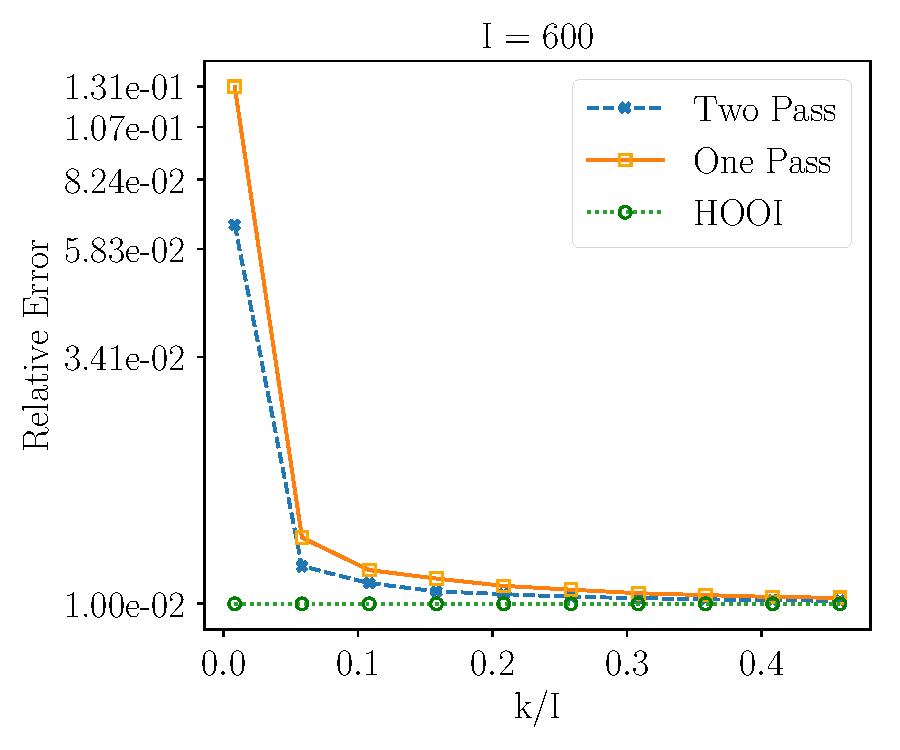
\includegraphics[scale = 0.3]{figure/id_lnoise_n600.pdf}
    \end{subfigure}
    \begin{subfigure}{0.32\textwidth}
    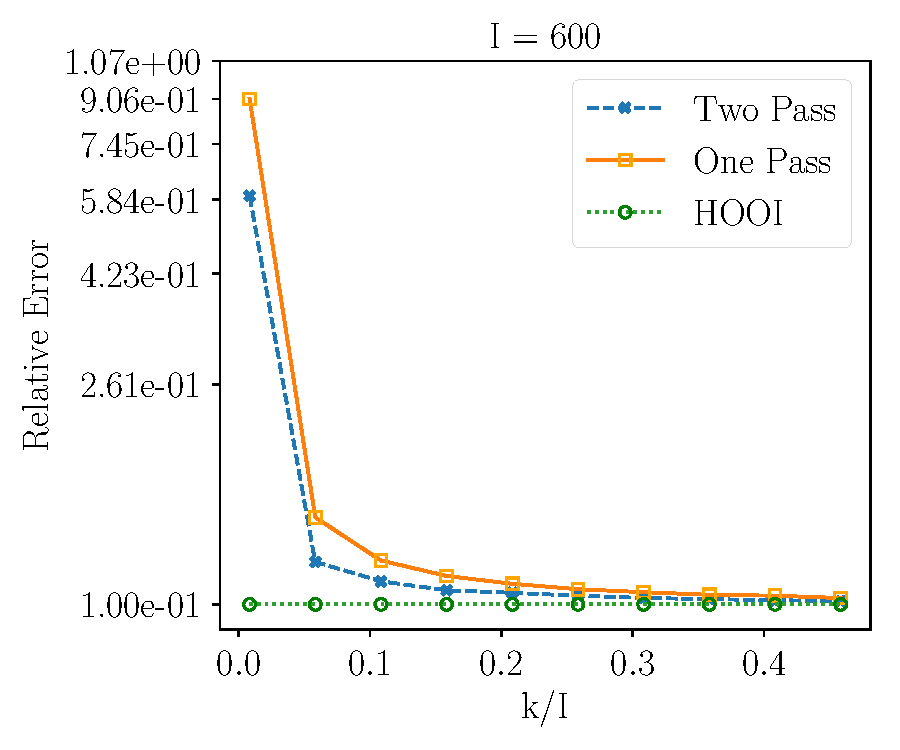
\includegraphics[scale = 0.3]{figure/id_mnoise_n600.pdf}
    \end{subfigure}
    \begin{subfigure}{0.32\textwidth}
    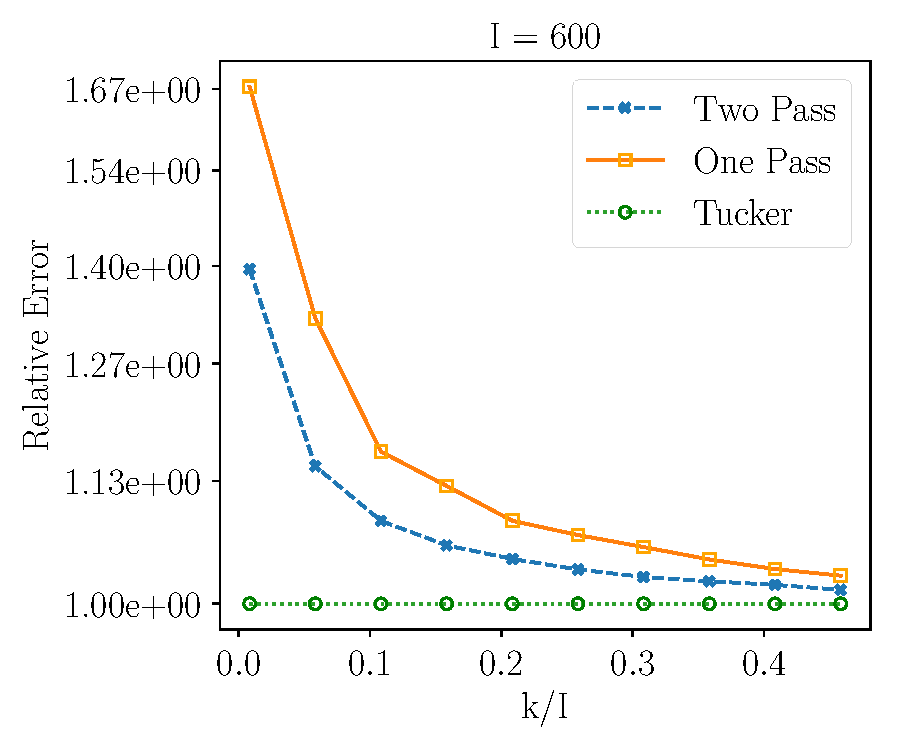
\includegraphics[scale = 0.3]{figure/id_hnoise_n600.pdf}
    \end{subfigure}
    \textbf{Superdiagonal +Low/Medium/High Noise ($\gamma = 0.01,0.1,1$)}
\caption{Relative error for fixed-rank tensor approximation as a function of the compression factor $k/n$: \textit{We compare the relative errors presented in log scale for two-pass sketching, one-pass sketching and Tucker decomposition for the input tensor with superdiagonal + noise design ($\gamma = 0.01,0.1,1$). Rank $r$ = 5.}} \label{fig:id_lnoise}
\end{figure}

\subsection{Application Examples}

For real-world application of our methods, we experimented on the state-of-the-art global climate simulation datasets based on the Community Earth System Model (CESM) Community Atmosphere Model (CAM) 5.0 \cite{hurrell2013community,kay2015community}. In particular, we used the dataset on aerosol absorption, which can affect climate through absorbing the solar radiation and changing cloud formation. This dataset recorded absorption at different times, altitudes, longitudes, and latitudes  ($240 \times 30 \times 192 \times 288$). Since the Tucker rank of the original tensor remains unknown, we compared different models for different choices of rank, with the result given in Figure \ref{fig:application}. Also, we performed additional experiments on the net surface radiative flux and dust aerosol burden data with the results given in Figure \ref{fig:srfrad}, \ref{fig:burden_dust} in Appendix \ref{appendix: more_real_data_result}. 
\begin{figure}[H] 
    \centering 
    \begin{subfigure}{0.31\textwidth}
    \end{subfigure}
    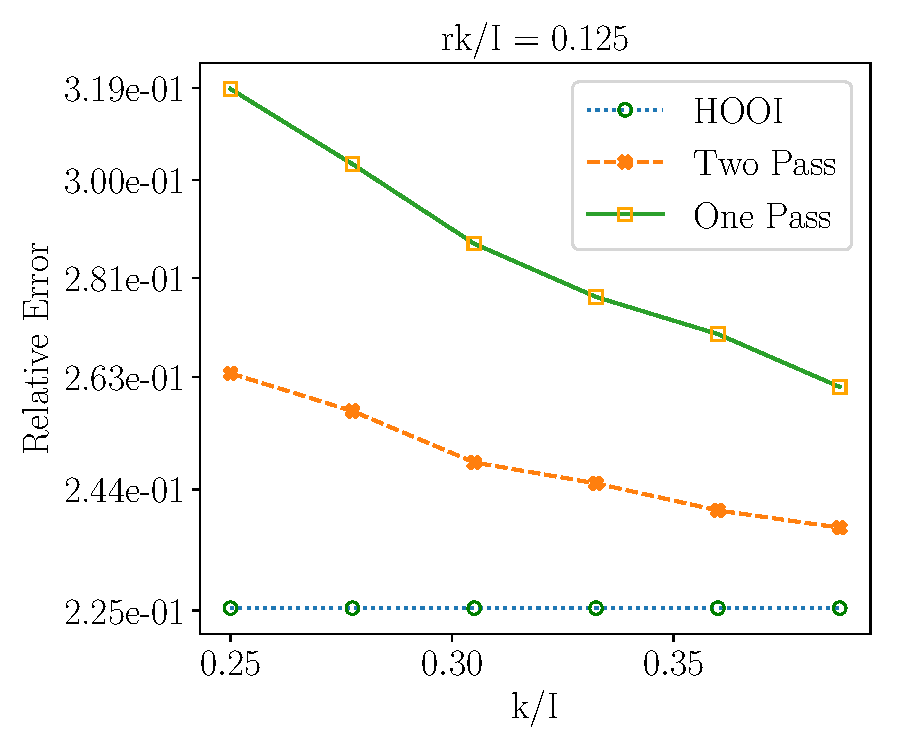
\includegraphics[scale = 0.29]{figure/ABSORB_frk8.pdf}
    \begin{subfigure}{0.31\textwidth}
    \end{subfigure}
    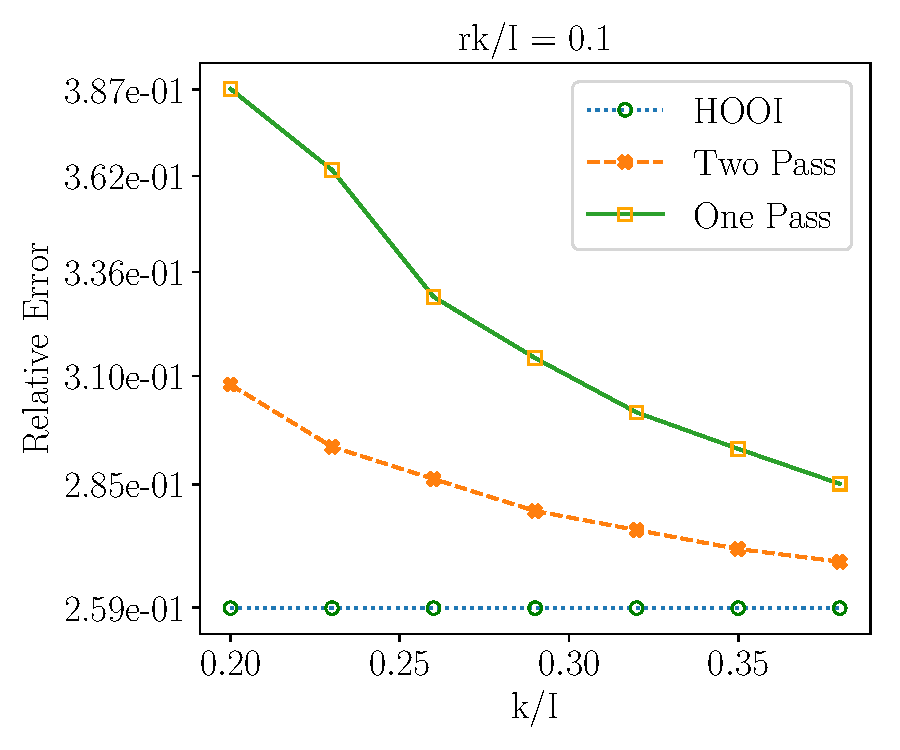
\includegraphics[scale = 0.29]{figure/ABSORB_frk10.pdf}
    \begin{subfigure}{0.31\textwidth}
    \end{subfigure}
    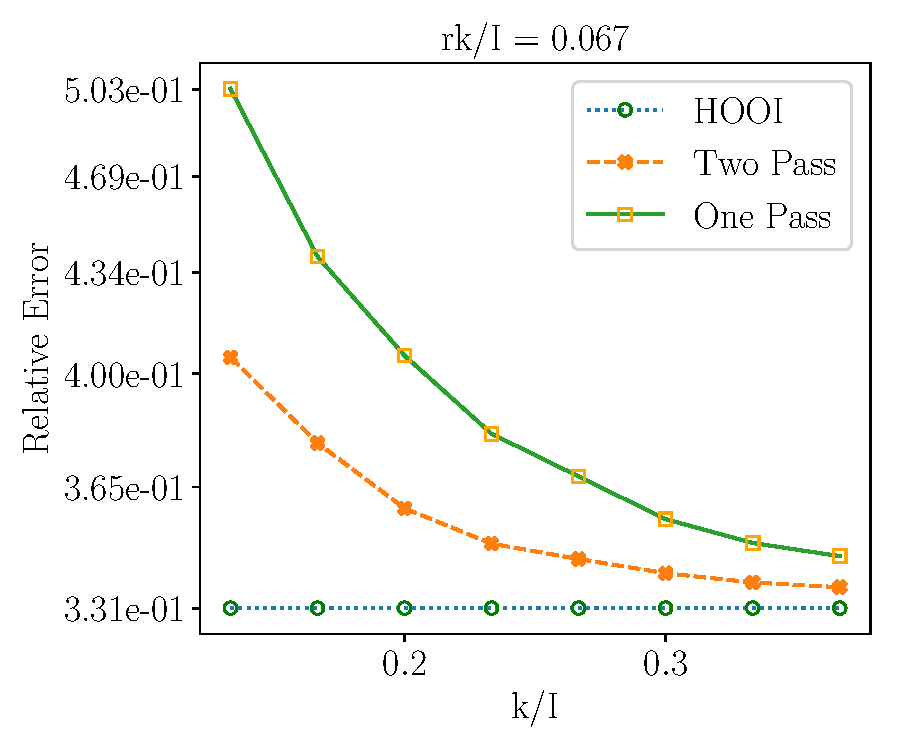
\includegraphics[scale = 0.29]{figure/ABSORB_frk15.pdf}
    \textbf{Aerosol Absorption}
\caption{Relative error for fixed-rank tensor approximation on climate simulation data ($240 \times 30 \times 192 \times 288$): \textit{We compared the relative errors presented in log scale for two-pass sketching, one-pass sketching and Tucker decomposition with different ranks ($rk/I = 0.125,0.2,0.067$).}} \label{fig:application}
\end{figure}

\section{Conclusion}

\newpage
\bibliographystyle{plain}
\bibliography{biblio}
\newpage 
\begin{appendices}
\section{Proof for Main Results}
\subsection{Proof for Theorem \ref{thm: low_rank_err}}
Let $\tilde{\mathscr{X}}$ denote the compressed tensor, 
\begin{equation}
\label{eq:definition_of_compression_tensor}
\tilde{\mathscr{X}} = \mathscr{X}\times_1  \mathbf{Q}_1\mathbf{Q}_1^\top \times_2 \cdots \times_N \mathbf{Q}_N\mathbf{Q}_N^\top.
\end{equation}
The error bound for $\hat{\mathscr{X}}_2$ from two pass algorithm follows directly from lemma \ref{lemma: compression_error} as the compression tensor is exactly the output of TwoPassLowRank in algorithm \ref{alg:two_pass_low_rank_appro}: $ \hat{\mathscr{X}}_2 = \tilde{\mathscr{X}}$. Now we turn to the proof for the one-pass algorithm. \par 
We claim that 
\begin{equation}
\label{eq:inner_zero}
\begin{aligned}
&\langle \hat{\mathscr{X}}_1 - \Tilde{\mathscr{X}}, \Tilde{\mathscr{X}} - \mathscr{X} \rangle = 0. 
\end{aligned}
\end{equation}
To see why, for $n \in [N]$, let 
\begin{equation} 
\label{eq:definition_Y_n}
\mathscr{Y}_n = \mathscr{X} \times_1 \mathbf{Q}_1\mathbf{Q}_1^\top \times_2 \cdots \times_n \mathbf{Q}_n\mathbf{Q}_n^\top,
\end{equation}
and $\mathscr{Y}_0 = \mathscr{X}$. 
Then 
\begin{equation}\label{eq: y_diff}
\begin{aligned}
\mathscr{X}-\tilde{\mathscr{X}} = \mathscr{Y}_0 - \mathscr{Y}_N= \sum_{n=0}^{N-1} (\mathscr{Y}_n - \mathscr{Y}_{n+1}).
\end{aligned}
\end{equation}
Besides, given the formula of $\hat{\mathscr{X}}_1$ in algorithm \ref{alg:one_pass_low_rank_appro} and the definition of $\tilde{\mathscr{X}}_1$, it is not hard to show that 
\begin{equation}
\begin{aligned}
\mathscr{\hat{X}}_1-\tilde{\mathscr{X}}= (\mathscr{W}-\mathscr{X}\times_1 \mathbf{Q}_1^\top \times_2 \cdots \times_N \mathbf{Q}_n^\top)  \times_1 \mathbf{Q}_1 \dots \times_N \mathbf{Q}_N. 
\end{aligned}
\end{equation}
For any $0\le n< N$, 
\begin{equation}
\mathscr{Y}_n-\mathscr{Y}_{n+1} = \mathscr{Y}_{n} \times_{n+1} (\mathbf{I} - \mathbf{Q}_{n+1}\mathbf{Q}^\top_{n+1}).
\end{equation}
Then with \label{eq:F_norm_equivalent}, 
\begin{equation}
\begin{aligned}
&\langle \mathscr{Y}_n-\mathscr{Y}_{n+1}, \hat{\mathscr{X}}_1-\tilde{\mathscr{X}}\rangle = \langle (\mathbf{I} - \mathbf{Q}_{n+1}\mathbf{Q}^\top_{n+1}) \mathbf{Y}_{n}^{n+1},  \mathbf{Q}_{n+1}\mathbf{B}_n^{(n+1)}\rangle \\
& = \rm{Tr}(\mathbf{Y}_{n}^{(n+1)} (\mathbf{I} - \mathbf{Q}_{n+1}\mathbf{Q}^\top_{n+1})\mathbf{Q}_{n+1}\mathbf{B}_n^{(n+1)} )=0 , 
\end{aligned}
\end{equation}
where $\mathbf{B}_n^{(n+1)}$ is the mode $(n+1)$th unfolding of tensor $\mathscr{B}_n$, $n \in [N]$, defined as 
\begin{equation}
\mathscr{B}_n = (\mathscr{W}-\mathscr{X}\times_1 \mathbf{Q}_1^\top \times \times_N \mathbf{Q}_n^\top)  \times_1 \mathbf{Q}_1 \dots \times_n \mathbf{Q}_n \times_{n+2}  \mathbf{Q}_{n+2} \dots \times_N   \mathbf{Q}_{N}. 
\end{equation}
Then \eqref{eq:inner_zero} indicates 
\begin{equation}
\label{eq:low_rank_decomposition}
 \mathbb{E}\| \hat{\mathscr{X}}_1 - \mathscr{X} \|_F^2 = \mathbb{E}\| \hat{\mathscr{X}}_1 - \Tilde{\mathscr{X}}\|_F^2 + \mathbb{E} \|\Tilde{\mathscr{X}} - \mathscr{X} \|_F^2. 
\end{equation}
Based the construction of $\hat{\mathscr{X}}_1$ and definition of $\mathscr{W}$ in algorithm \ref{alg:one_pass_low_rank_appro}, 
\begin{equation}
\begin{aligned}
&\mathbb{E} \|\hat{\mathscr{X}}_1 - \tilde{\mathscr{X}}\|^2_F = 
\mathbb{E}\|(\mathscr{W} - \mathscr{X}\times_1 \mathbf{Q}_1^\top \cdots \times_N \mathbf{Q}^\top_N)\times_1 \mathbf{Q}_1\cdots \times_N \mathbf{Q}_N \|^2_F\\
& = \mathbb{E}\|(\mathscr{W} - \mathscr{X}\times_1 \mathbf{Q}_1^\top \cdots \times_N \mathbf{Q}^\top_N)\|_F^2,  \end{aligned}
\end{equation}
where we use the fact that the mode product with an orthogonal matrix will not change the value of Frobenius norm. 

Applying the probabilistic error bound in lemma \ref{lemma: compression_error} for the second term in \eqref{eq:low_rank_decomposition} and applying probabilistic error bound in lemma \ref{lemma:err_core_sketch} into above equation, 
taking minimum among $1\le \rho <k-1$ we could finish proof. 
\subsection{Proof for Corollary \ref{corollary:fix_rank_err}}
Follow the argument in the proof for Proposition 7.1 in \cite{tropp2017practical}, we could get 
\begin{equation}
\begin{aligned}
&\|\mathscr{X} - \llbracket \hat{\mathscr{X}}_2 \rrbracket_\mathbf{r}\|_F \le \|\mathscr{X} -  \hat{\mathscr{X}}_2\|_F+\|\hat{\mathscr{X}}_2 -  \llbracket\hat{\mathscr{X}}_2\rrbracket_\mathbf{r}\|_F\\
&\le \|\mathscr{X} -  \hat{\mathscr{X}}_2\|_F+\|\hat{\mathscr{X}}_2 -  \llbracket \mathscr{X}\rrbracket_\mathbf{r}\|_F \\
&\le 2\|\mathscr{X} - \hat{\mathscr{X}}_2 \|_F + \|\mathscr{X} -  \llbracket \mathscr{X} \rrbracket_\mathbf{r}\|_F.
\end{aligned}
\end{equation}
The first and the third line follow from the trangle inequality and the second line follow from the definition of best rank $r$ approximation. Then taking the expectation, applying the result of theorem \ref{thm: low_rank_err} and using the fact $\mathbb{E} y^2 \ge (\mathbb{E} |y|)^2$ for any random variable $y$, we could finish the proof. And with the same argument, we could show the probabilistic error bound for $\llbracket\hat{\mathscr{X}}_1\rrbracket_\mathbf{r}$.


\section{Probabilistic Analysis of the Compression Error}
First, we establish a bound for the expected error at the compression stage. Let $\tilde{\mathscr{X}}$ follow the definition in \eqref{eq:definition_of_compression_tensor}.
\begin{lem}
\label{lemma: compression_error}
For any natural number $\rho<k-1$,
\begin{equation}
\mathbb{E}  \|\tilde{\mathscr{X}} - \mathscr{X}\|_F \le \sum_{n=1}^N \left(1+\frac{\rho}{k-\rho-1}\right)(\tau^{(n)}_\rho)^2. 
\end{equation}

\begin{proof}
The main idea of the proof is to extend the result of \cite{halko2011finding} to the tensor case. To construct similar bound, we first decompose the compression error into the sum of differences between $\mathscr{Y}_m$ as in \eqref{eq: y_diff}, and then bound each term individually as in \eqref{eq: y_diff_bound}.

Follow the definition of $\mathscr{Y}_n$ in \ref{eq:definition_Y_n}, 
\begin{equation}\label{eq: y_diff}
\begin{aligned}
& \|\mathscr{X}-\tilde{\mathscr{X}}\|_F^2 = \|\mathscr{Y}_0 - \mathscr{Y}_N\|_F^2= \|\sum_{n=0}^{N-1} (\mathscr{Y}_n - \mathscr{Y}_{n+1})\|_F^2.
\end{aligned}
\end{equation}
For any $0\le m< n < N$, 
\begin{equation}
\mathscr{Y}_m-\mathscr{Y}_{m+1} = \mathscr{Y}_{m} \times_{(m+1)} (\mathbf{I} - \mathbf{Q}_{m+1}\mathbf{Q}^\top_{m+1}). 
\end{equation}
and 
\begin{equation}
\begin{aligned}
&\mathscr{Y}_n - \mathscr{Y}_{n+1}  = \underbrace{\left[\mathscr{X}\times_1 \mathbf{Q}_{1}\mathbf{Q}^\top_{1} \times_2 \cdots \times_{m} \mathbf{Q}_{m}\mathbf{Q}^\top_{m}\times_{(m+2)} \cdots  \times_{n} \mathbf{Q}_{n}\mathbf{Q}^\top_{n}\times_{(n+1)}(\mathbf{I}-\mathbf{Q}_{(n+1)}\mathbf{Q}^\top_{(n+1)})\right]}_{\mathscr{A}}\\
&\times_{(m+1)} \mathbf{Q}_{m+1}\mathbf{Q}^\top_{m+1}.
\end{aligned}
\end{equation}
Then second part of lemma \ref{lemma:projection_tensors} claims that 
\begin{equation}\label{eq:inner_prod1}
\langle\mathscr{Y}_m-\mathscr{Y}_{m+1},  \mathscr{Y}_n - \mathscr{Y}_{n+1}\rangle = \langle\mathscr{Y}_{m} \times_{(m+1)} (\mathbf{I} - \mathbf{Q}_{m+1}\mathbf{Q}^\top_{m+1}), \mathscr{A} \times_{m+1} \mathbf{Q}_{m+1}\mathbf{Q}^\top_{m+1} \rangle = 0.
\end{equation}
It indicates that we could decompose error with the Pythagorean Theorem as:  
\begin{equation}
\label{eq:comression_decomposition}
\begin{aligned}
& \|\mathscr{X}-\tilde{\mathscr{X}}\|_F^2 =  \sum_{n=0}^{N-1} \| (\mathscr{Y}_n - \mathscr{Y}_{n+1})\|_F^2.
\end{aligned}
\end{equation}
Now we shall bound $\|\mathscr{Y}_n - \mathscr{Y}_{n+1}\|_F^2$ for each $n$.   
\begin{equation} \label{eq: y_diff_bound}
\begin{aligned}
&\|\mathscr{Y}_n - \mathscr{Y}_{n+1}\|_F^2 = \|\mathscr{X}\times_{(n+1)} (\mathbf{I} - \mathbf{Q}_{n+1}\mathbf{Q}_{n+1}^\top)\times_{1} \mathbf{Q}_{1}\mathbf{Q}_{1}^\top\dots \times_n \mathbf{Q}_{n}\mathbf{Q}_{n}^\top\|_F^2 \\
&\le \|\mathscr{X}\times_{(n+1)} (\mathbf{I} - \mathbf{Q}_{n+1}\mathbf{Q}_{n+1}^\top)\|_F^2 \\
&= \| (\mathbf{I} - \mathbf{Q}_{n+1}\mathbf{Q}_{n+1}^\top)\mathbf{X}^{(n)}\|_F^2,
\end{aligned}
\end{equation}
where the second line follows from the fact that the projection is contractive with second part in lemma \ref{lemma:projection_tensors}. 
Applying lemma \ref{lemma:sketchy_column_space_err} to last line of above inequality, we could show that 
\begin{equation}
\mathbb{E} \|\mathscr{Y}_n - \mathscr{Y}_{n+1}\|_F^2 \le \left(1+\frac{\rho}{k-\rho-1}\right)(\tau^{(n+1)}_\rho)^2.
\end{equation}
Sum all the upper bounds up for each term in  \eqref{eq:comression_decomposition}, we finish the proof. 
\end{proof}
\end{lem}
\section{Probabilistic Analysis of Linkage Tensor}
We first introduce a lemma which may assist us to apply lemma \ref{lemma:expectation_inverse_gaussian} in lemma \ref{lemma:probabilistic_err_linkage_tensor}. 
\begin{lem}
\label{lemma:indepence_for_pseduo_inverse}
Follow the definition of $\mathbf{\Omega}_n$ and $\mathbf{Q}_n$, 
for any $1\le n\le N$, $\mathbf{\Phi}_n \mathbf{Q}_n$ and 
$\mathbf{\Phi}_n (\mathbf{I} - \mathbf{Q}_n\mathbf{Q}_n^\top)$ are conditional independent given $\mathbf{Q}_n$. 
\begin{proof}
Considering both $(\mathbf{\Phi}_n \mathbf{Q}_n)$ and $(\mathbf{\Phi}_n (\mathbf{I} -\mathbf{Q}_n\mathbf{Q}_n^\top))$ are both Gaussian matrix, it suffices to show that covariance matrix between $\mbox{vec}(\mathbf{\Phi}_n \mathbf{Q}_n)$ and $\mbox{vec}(\mathbf{\Phi}_n (\mathbf{I} -\mathbf{Q}_n\mathbf{Q}_n^\top))$ with $\mathbf{Q}_n$ fixed, is the identity. Note: $\mbox{vec}(AB) = (B^\top \otimes I)\mbox{vec}(A)$. 
\begin{equation}
\begin{aligned}
&\cov(\mbox{vec}(\mathbf{\Phi}_n \mathbf{Q}_n), \mbox{vec}(\mathbf{\Phi}_n (\mathbf{I} -\mathbf{Q}_n\mathbf{Q}_n^\top)))  = \left(\mathbf{Q}_n^\top \otimes \mathbf{I}_k\right)\left((\mathbf{I} - \mathbf{Q}\mathbf{Q}_n^\top) \otimes \mathbf{I}_k\right)\\
&=\left(\mathbf{Q}_n^\top(\mathbf{I} - \mathbf{Q}_n\mathbf{Q}_n^\top)  \right)\otimes \left(\mathbf{I}_k\right) = \mathbf{I}_{k^2} 
\end{aligned}
\end{equation}
completes the proof. 
\end{proof}
\end{lem}

\begin{lem}
\label{lemma:probabilistic_err_linkage_tensor}
\begin{equation}
\mathbb{E} \|\mathscr{W} - \mathscr{X}\times_1 \mathbf{Q}_1^\top \times \cdots \times_N \mathbf{Q}_N^\top\|_F^2\le 
\left(1+\frac{k}{s-k}\right)^N  \sum_{n=1}^N \left(1+\frac{k}{k-\rho-1}\right)(\tau^{(n)}_\rho)^2. 
\end{equation}
\begin{proof}
To make notation succinct, we borrow the concept and notation of filtration in probability:
\begin{equation}
\mathcal{F}_n = \sigma(\mathbf{\Omega}_1, \mathbf{\Phi}_1, \dots, \mathbf{\Omega}_n, \mathbf{\Phi}_n), 
\end{equation}
where $\sigma(\mathbf{\Omega}_1, \mathbf{\Phi}_1, \dots, \mathbf{\Omega}_n, \mathbf{\Phi}_n)$ is the sigma algebra generated by $\{\mathbf{\Omega}_i, \mathbf{\Phi}_i, 1\le i\le n\}$. Let $\mathcal{F}_0 = \{\Omega, \emptyset\}$,  the trivial sigma algebra. Here $\Omega$ is the whole space. In usage, it just simplifies writing the conditional probability:
\begin{equation}
\mathbb{E} (X \mid \mathcal{F}_n) = \mathbb{E} (X\mid \mathbf{Q}_1,\mathbf{\Omega}_1, \dots, \mathbf{Q}_n,\mathbf{\Omega}_n). 
\end{equation}

\begin{equation}
\begin{aligned}
&\mathscr{W} = \mathscr{Z}\times_1 (\mathbf{\Phi}_1 \mathbf{Q}_1)^\dag \times \cdots \times_N (\mathbf{\Phi}_N \mathbf{Q}_N)^\dag \\
& = (\mathscr{X} -  \tilde{\mathscr{X}})\times_1 \mathbf{\Phi}_1 \times \cdots \times_N \mathbf{\Phi}_N  \times_1 (\mathbf{\Phi}_1 \mathbf{Q}_1)^\dag \times \cdots \times_N (\mathbf{\Phi}_N \mathbf{Q}_N)^\dag 
\\
&+ \tilde{\mathscr{X}}\times_1 \mathbf{\Phi}_1 \times \cdots \times_N \mathbf{\Phi}_N \times_1 (\mathbf{\Phi}_1 \mathbf{Q}_1)^\dag \times \cdots \times_N (\mathbf{\Phi}_N \mathbf{Q}_N)^\dag.
\end{aligned}
\end{equation}
Noticing 
\begin{equation}
\begin{aligned}
&\tilde{\mathscr{X}}\times_1 \mathbf{\Phi}_1 \times \cdots \times_N \mathbf{\Phi}_N \times_1 (\mathbf{\Phi}_1 \mathbf{Q}_1)^\dag \times \cdots \times_N (\mathbf{\Phi}_N \mathbf{Q}_N)^\dag   \\
& = \mathscr{X}\times_1 (\mathbf{\Phi}_1 \mathbf{Q}_1)^\dag \mathbf{\Phi}_1\mathbf{Q}_1\mathbf{Q}_1^\top \times \cdots \times_N (\mathbf{\Phi}_N \mathbf{Q}_N)^\dag \mathbf{\Phi}_N\mathbf{Q}_N\mathbf{Q}_N^\top\\
& = \mathscr{X}\times_1 \mathbf{Q}_1^\top \times \cdots \times_N \mathbf{Q}_N^\top.
\end{aligned}
\end{equation}
The last equation comes from the fact that for a matrix $\mathbf{A}$ with shape $s\times k$, if $s>k$, $A^\dag A = I_k$. Therefore
\begin{equation}
\begin{aligned}
&\mathscr{W} = (\mathscr{X} -  \tilde{\mathscr{X}})\times_1 \mathbf{\Phi}_1 \times \cdots \times_N \mathbf{\Phi}_N  \times_1 (\mathbf{\Phi}_1 \mathbf{Q}_1)^\dag \times \cdots \times_N (\mathbf{\Phi}_N \mathbf{Q}_N)^\dag \\
&+ \mathscr{X}\times_1 \mathbf{Q}_1^\top \times \cdots \times_N \mathbf{Q}_N^\top.
\end{aligned}
\end{equation}
Now it suffices to bound the first term in above equation. Applying \eqref{eq: tensor_product_mul_exchangable} and \eqref{eq: tensor_product_association}, we could rearrange first part as
\begin{equation}
\begin{aligned}
&(\mathscr{X} -  \tilde{\mathscr{X}})\times_1 \mathbf{\Phi}_1 \times \cdots \times_N \mathbf{\Phi}_N  \times_1 (\mathbf{\Phi}_1 \mathbf{Q}_1)^\dag \times \cdots \times_N (\mathbf{\Phi}_N \mathbf{Q}_N)^\dag \\
& =(\mathscr{X} -  \tilde{\mathscr{X}})\times_1 (\mathbf{\Phi}_1\mathbf{Q}_1)^\dag \mathbf{\Phi}_1 \times \cdots \times_N (\mathbf{\Phi}_N\mathbf{Q}_N)^\dag \mathbf{\Phi}_N.
\end{aligned}
\end{equation}
We use a recursive argument to bound above equation. Let 
$\mathscr{Y}_0 = (\mathscr{X} -  \tilde{\mathscr{X}})$ and for $1\le n \le N$, 
\begin{equation}
\mathscr{Y}_n =  (\mathscr{X} -  \tilde{\mathscr{X}})\times_1 (\mathbf{\Phi}_1\mathbf{Q}_1)^\dag \mathbf{\Phi}_1 \times \cdots \times_n (\mathbf{\Phi}_n\mathbf{Q}_n)^\dag \mathbf{\Phi}_n.
\end{equation}
For $0\le n<N$, 
\begin{equation}
\label{eq:recursion}
\mathbb{E} [\|\mathscr{Y}_{n+1}\|_F^2] = \mathbb{E}\left\{ \mathbb{E} [\|\mathscr{Y}_{n+1}\|_F^2 \mid \mathcal{F}_n] \right\} = \mathbb{E} \left\{\mathbb{E}_{\mathbf{Q}_{n+1}, \mathbf{\Omega}_{n+1}}  \|\mathscr{Y}_n\times_{(n+1)}\right (\mathbf{\Phi}_{n+1}\mathbf{Q}_{n+1})^\dag \mathbf{\Phi}_{n+1}\|_F^2\}. 
\end{equation}
Here, we use the fact that $\mathbf{Q}_{n+1}$ only depends on $\mathbf{\Omega}_{n+1}$. Noticing $\mathscr{Y}_n$, $\mathbf{\Phi}_{n+1}$ and $\mathbf{Q}_{n+1}$ are independent with each other, 

\begin{equation}
\label{eq:conditional_recursion}
\begin{aligned}
&\mathbb{E}_{\mathbf{Q}_{n+1}, \mathbf{\Omega}_{n+1}}  \|\mathscr{Y}_n\times_{(n+1)} (\mathbf{\Phi}_{n+1}\mathbf{Q}_{n+1})^\dag \mathbf{\Phi}_{n+1}\|_F^2\\
& = \mathbb{E}_{\mathbf{Q}_{n+1}, \mathbf{\Omega}_{n+1}} \|(\mathbf{\Phi}_{n+1}\mathbf{Q}_{n+1})^\dag \mathbf{\Phi}_{n+1} \mathbf{Y}_n^{(n+1)}\|_F^2\\
& = \mathbb{E}_{\mathbf{Q}_{n+1}, \mathbf{\Omega}_{n+1}} \|(\mathbf{\Phi}_{n+1}\mathbf{Q}_{n+1})^\dag \mathbf{\Phi}_{n+1}(\mathbf{Q}_{n+1}\mathbf{Q}_{n+1}^\top +\mathbf{I}-\mathbf{Q}_{n+1}\mathbf{Q}_{n+1}^\top ) \mathbf{Y}_n^{(n+1)}\|_F^2\\
& = \mathbb{E}_{\mathbf{Q}_{n+1}, \mathbf{\Omega}_{n+1}} \|(\mathbf{\Phi}_{n+1}\mathbf{Q}_{n+1})^\dag \mathbf{\Phi}_{n+1}(\mathbf{Q}_{n+1}\mathbf{Q}_{n+1}^\top)\mathbf{Y}_n^{(n+1)}\|_F^2\\
&+\mathbb{E}_{\mathbf{Q}_{n+1}, \mathbf{\Omega}_{n+1}} \|(\mathbf{\Phi}_{n+1}\mathbf{Q}_{n+1})^\dag \mathbf{\Phi}_{n+1}(\mathbf{I}-\mathbf{Q}_{n+1}\mathbf{Q}_{n+1}^\top)\mathbf{Y}_n^{(n+1)}\|_F^2\\
&+2\mathbb{E}_{\mathbf{Q}_{n+1}, \mathbf{\Omega}_{n+1}}  \langle(\mathbf{\Phi}_{n+1}\mathbf{Q}_{n+1})^\dag \mathbf{\Phi}_{n+1}(\mathbf{Q}_{n+1}\mathbf{Q}_{n+1}^\top)\mathbf{Y}_n^{(n+1)},  (\mathbf{\Phi}_{n+1}\mathbf{Q}_{n+1})^\dag \mathbf{\Phi}_{n+1}(\mathbf{I}-\mathbf{Q}_{n+1}\mathbf{Q}_{n+1}^\top)\mathbf{Y}_n^{(n+1)}\rangle. 
\end{aligned}
\end{equation}
Since $\mathbf{Q}_{n+1}$ is independent of $\mathbf{\Omega}_{n+1}$, the last line in \ref{eq:conditional_recursion} becomes 
\begin{equation}
\begin{aligned}
&\mathbb{E}_{\mathbf{Q}_{n+1}, \mathbf{\Omega}_{n+1}}  \langle\mathbf{Q}_{n+1}^\top\mathbf{Y}_n^{(n+1)},  (\mathbf{\Phi}_{n+1}\mathbf{Q}_{n+1})^\dag \mathbf{\Phi}_{n+1}(\mathbf{I}-\mathbf{Q}_{n+1}\mathbf{Q}_{n+1}^\top)\mathbf{Y}_n^{(n+1)}\rangle\\
&= \mathbb{E}_{\mathbf{Q}_{n+1}} \langle\mathbf{Q}_{n+1}^\top\mathbf{Y}_n^{(n+1)}, \mathbb{E}_{\mathbf{\Omega}_{n+1}}  (\mathbf{\Phi}_{n+1}\mathbf{Q}_{n+1})^\dag \mathbf{\Phi}_{n+1}(\mathbf{I}-\mathbf{Q}_{n+1}\mathbf{Q}_{n+1}^\top)\mathbf{Y}_n^{(n+1)} \mid \mathbf{Q}_{n+1}\rangle. 
\end{aligned}
\end{equation}



Now lemma \ref{lemma:indepence_for_pseduo_inverse} claims that $\mathbf{\Phi}_n\mathbf{Q}_n$ and $\mathbf{\Phi}_n(\mathbf{I} - \mathbf{Q}_n\mathbf{Q}_n^\top)$ are independent given $\mathbf{Q}_n$. Besides, 
$\mathbb{E} \mathbf{\Phi}_{n+1}(\mathbf{I}-\mathbf{Q}_{n+1}\mathbf{Q}_{n+1}^\top )\mid \mathbf{Q}_{n+1} = 0$, then above equation becomes zero. \par 
The fact that the expectation of inner product is zero leads to another Pythagorean Theorem type decomposition of \ref{eq:conditional_recursion} as
\begin{equation}
\begin{aligned}
&\mathbb{E}_{\mathbf{Q}_{n+1}, \mathbf{\Omega}_{n+1}}  \|\mathscr{Y}_n\times_{(n+1)} (\mathbf{\Phi}_{n+1}\mathbf{Q}_{n+1})^\dag \mathbf{\Phi}_{n+1}\|_F^2\\
& = \mathbb{E}_{\mathbf{Q}_{n+1}, \mathbf{\Omega}_{n+1}} \|(\mathbf{\Phi}_{n+1}\mathbf{Q}_{n+1})^\dag \mathbf{\Phi}_{n+1}(\mathbf{Q}_{n+1}\mathbf{Q}_{n+1}^\top)\mathbf{Y}_n^{(n+1)}\|_F^2\\
&+\mathbb{E}_{\mathbf{Q}_{n+1}, \mathbf{\Omega}_{n+1}} \|(\mathbf{\Phi}_{n+1}\mathbf{Q}_{n+1})^\dag \mathbf{\Phi}_{n+1}(\mathbf{I}-\mathbf{Q}_{n+1}\mathbf{Q}_{n+1}^\top)\mathbf{Y}_n^{(n+1)}\|_F^2.\\
\end{aligned}
\end{equation}
Since $s>k$, $(\mathbf{\Phi}_{n+1}\mathbf{Q}_{n+1})^\dag \mathbf{\Phi}_{n+1}\mathbf{Q}_{n+1} = \mathbf{I}_k$, 
\begin{equation}
\|(\mathbf{\Phi}_{n+1}\mathbf{Q}_{n+1})^\dag \mathbf{\Phi}_{n+1}(\mathbf{Q}_{n+1}\mathbf{Q}_{n+1}^\top)\mathbf{Y}_n^{(n+1)}\|_F^2 = \|\mathbf{Q}_{n+1}^\top\mathbf{Y}_n^{(n+1)}\|_F^2 \le \|\mathbf{Y}_n^{(n+1)}\|_F^2.
\end{equation}
 For the second part, let $\mathbf{B}_{1,n+1} = (\mathbf{\Phi}_{n+1}\mathbf{Q}_{n+1})^\dag$, $\mathbf{B}_{2,n+1} = \mathbf{\Phi}_{n+1}(\mathbf{I}-\mathbf{Q}_{n+1}\mathbf{Q}_{n+1}^\top)$, 
 as we show above, each element in $\mathbf{B}_{1,n+1}$ is independent from each element in $\mathbf{B}_{2,n+1}$. Then 
\begin{equation}
\begin{aligned}
&\mathbb{E}_{\mathbf{Q}_{n+1}, \mathbf{\Omega}_{n+1}} \|(\mathbf{\Phi}_{n+1}\mathbf{Q}_{n+1})^\dag \mathbf{\Phi}_{n+1}(\mathbf{I}-\mathbf{Q}_{n+1}\mathbf{Q}_{n+1}^\top)\mathbf{Y}_n^{(n+1)}\|_F^2\\
& =\mathbb{E}_{\mathbf{Q}_{n+1}} \mathbb{E}_{\mathbf{B}_{1,n+1}, \mathbf{B}_{2, n+1}} \|\mathbf{B}_{1,n+1}^\dag
\mathbf{B}_{2,n+1}\mathbf{Y}_n^{(n+1)}\|_F^2\\
& = \frac{k}{s-k}\|\mathbf{Y}_n^{(n+1)}\|_F^2.
\end{aligned}
\end{equation}
Then we get a recursive relation as 
\begin{equation}
\mathbb{E}\|\mathscr{Y}_{n}\|_F^2 \le  \left(1+\frac{k}{s-k}\right) \mathbb{E}\|\mathscr{Y}_{n-1}\|_F^2, n\ge 1, 
\end{equation}
which leads to 
\begin{equation}
\mathbb{E}\|\mathscr{Y}_{N}\|_F^2 \le  \left(1+\frac{k}{s-k}\right)^N  \mathbb{E}\|\mathscr{Y}_0\|_F^2 \le  \left(1+\frac{k}{s-k}\right)^N  \sum_{n=1}^N \left(1+\frac{k}{k-\rho-1}\right)(\tau^{(n)}_\rho)^2, 
\end{equation}
where the last inequality comes from lemma \ref{lemma: compression_error}. 
\end{proof}
\end{lem}
\section{Proof for Lemma \ref{lemma: equivalance_one_pass}}
\begin{proof} 
First we claim there exists one best rank $\mathbf{r}$ tucker decomposition(there may be more than one optimal solutions),
\begin{equation}
 \llbracket \mathscr{W}\times_1 \mathbf{Q}_1 \cdots \times_N \mathbf{Q}_N \rrbracket_\mathbf{r} = \mathscr{S} \times_1 \mathbf{U}_1 \cdots \times_N \mathbf{U}_N,
\end{equation}
where $\mathbf{Q}_n \in \mathbb{R}^{k\times I_n}, \mathbf{U}_n \in \mathbb{R}^{r\times I_n}, n\in [N]$, $\mathscr{W}\in \mathbb{R}^{k^N}$ and $\mathscr{S}\in \mathbb{R}^{s^N}$, such that $\rm{Col}(\mathbf{U}_n) \subseteq \rm{Col}(\mathbf{Q}_n)$, for all $n \in [N]$. Here $\rm{Col}(\mathbf{U}_n)$ denotes the column of space of $\mathbf{U}_n$: the space spanned from columns of $\mathbf{U}_n$. Our argument is that given a solution $\llbracket \mathscr{S}; \mathbf{U}_n, n\in [N]\rrbracket$, $\llbracket \mathscr{S}; \mathbf{U}_n^{\mathbf{Q}_n}\mathbf{Q}_n^\top, n\in [N]\rrbracket$  is also a solution to the optimization problem \eqref{eq:tucker_optimization} i.e., 
\begin{equation}
\mathscr{S} \times_1 \mathbf{U}_1^{\mathbf{Q}_1}\mathbf{Q}_1^\top\times_2 \cdots \times_N \mathbf{U}_N^{\mathbf{Q}_N}\mathbf{Q}_N^\top = \mathscr{S} \times_1 \mathbf{U}_1\times \cdots \times_N \mathbf{U}_N, 
\end{equation}
where $\mathbf{U}_n^{\mathbf{Q}_n}$ and $\mathbf{U}_n^{\mathbf{Q}^\bot_n}$ follow the notations in proof of lemma \ref{lemma:err_core_sketch}.
It suffices to show that we could replace $\mathbf{U}_1$ with
$\mathbf{U}_1^{\mathbf{Q}_1}\mathbf{Q}_1^\top$ still attaining the solution to optimization problem \eqref{eq:tucker_optimization} and rest follows with the same argument. Rewriting identity matrix, 
\begin{equation}
\begin{aligned}
&\|\mathscr{W}\times_1 \mathbf{Q}_1 \cdots \times_N \mathbf{Q}_N - \mathscr{S} \times_1 \mathbf{U}_1 \cdots \times_N \mathbf{U}_N\|_F^2 \\
& = \|\mathscr{W}\times_1 \mathbf{Q}_1 \cdots \times_N \mathbf{Q}_N - \mathscr{S} \times_1[ \mathbf{U}_1^{\mathbf{Q}_1}\mathbf{Q}_1^\top+\mathbf{U}_1^{\mathbf{Q}^\bot_1}(\mathbf{Q}^\bot_1)^\top  ]\times_2\cdots \times_N \mathbf{U}_N\|_F^2.
\end{aligned}
\end{equation}
Similar to the trick in \eqref{eq:inner_prod1} and \eqref{eq:inner_prod2}, $\forall n_1, n_2 \in [N]$, 
\begin{equation}
\begin{aligned}
&\langle \mathscr{W}\times_1 \mathbf{Q}_1 \cdots \times_N \mathbf{Q}_N,\mathscr{S} \times_1 \cdots \times_{n_1} (\mathbf{U}_{n_1}^{\mathbf{Q}^\bot_{n_1}}(\mathbf{Q}^\bot_{n_1})^\top)\cdots \times_N \mathbf{U}_N \rangle =0 \\
& \langle \mathscr{S} \times_1 \cdots \times_{n_1} (\mathbf{U}_{n_1}^{\mathbf{Q}_{n_1}}\mathbf{Q}_{n_1}^\top)\times_2\cdots \times_N \mathbf{U}_N, \mathscr{S} \times_1 \cdots \times_{n_2} (\mathbf{U}_{n_2}^{\mathbf{Q}^\bot_{n_2}}(\mathbf{Q}^\bot_{n_2})^\top)\cdots \times_N \mathbf{U}_N \rangle =0,
\end{aligned}
\end{equation}
which indicates that 
\begin{equation}
\begin{aligned}
&\|\mathscr{W}\times_1 \mathbf{Q}_1 \cdots \times_N \mathbf{Q}_N - \mathscr{S} \times_1 \mathbf{U}_1 \cdots \times_N \mathbf{U}_N\|_F^2 \\
& = \|\mathscr{W}\times_1 \mathbf{Q}_1 \cdots \times_N \mathbf{Q}_N - \mathscr{S} \times_1 (\mathbf{U}_1^{\mathbf{Q}_1}\mathbf{Q}_1^\top) \cdots \times_N \mathbf{U}_N\|_F^2\\
& + \|\mathscr{S} \times_1 (\mathbf{U}_1^{\mathbf{Q}^\bot_1}(\mathbf{Q}^\bot_1)^\top) \cdots \times_N \mathbf{U}_N\|_F^2.
\end{aligned}
\end{equation}
By definition of minimizer, we could claim
\begin{equation}
\begin{aligned}
&\|\mathscr{W}\times_1 \mathbf{Q}_1 \cdots \times_N \mathbf{Q}_N - \mathscr{S} \times_1 \mathbf{U}_1 \cdots \times_N \mathbf{U}_N\|_F^2 \\
&= \|\mathscr{W}\times_1 \mathbf{Q}_1 \cdots \times_N \mathbf{Q}_N - \mathscr{S} \times_1 (\mathbf{U}_1^{\mathbf{Q}_1}\mathbf{Q}_1^\top ) \cdots \times_N \mathbf{U}_N\|_F^2\\
\end{aligned}
\end{equation}
which completes the argument.\par 
Then we could assume $\mathbf{U}_n = \mathbf{G}_n\mathbf{Q}_n$, where both $\mathbf{G}_n \in \mathbb{R}^{r\times k}$and $ \mathbf{Q}_n \in \mathbb{R}^{k\times I_n}$ are orthogonal matrices. The optimization problem becomes:
\begin{equation}
\begin{aligned}
&\min_{\mathscr{G}, \mathbf{G}_n} \|\mathscr{W}\times_1 \mathbf{Q}_1 \times_2\cdots \times_N \mathbf{Q}_N-\mathscr{G}\times_1 \mathbf{G}_1\mathbf{Q}_1 \times_2\cdots \times_N \mathbf{G}_N\mathbf{Q}_N\|_F^2\\
& s.t. \quad \mathbf{G}_n^\top \mathbf{G}_n = \mathbf{I}_{r\times r}, \quad n \in [N].
\end{aligned}
\end{equation}
Noticing that the mode product with an orthogonal matrix does not change the Frobenius norm and exchanging rule of mode product \eqref{eq: tensor_product_mul_exchangable}, we could further simply the optimization problem to 
\begin{equation}
\begin{aligned}
&\min_{\mathscr{G}, \mathbf{G}_n} \|\mathscr{W}-\mathscr{G}\times_1 \mathbf{G}_1 \times_2\cdots \times_N \mathbf{G}_N\|_F^2\\
& s.t. \quad \mathbf{G}_n^\top \mathbf{G}_n = \mathbf{I}_{r\times r}, \quad n \in [N],
\end{aligned}
\end{equation}
which completes the proof. 
\end{proof}
\section{Technical Lemmas}
\subsection{Technical Lemmas for sketching Matrix}
All the proof for lemmas in this section could be found in chapter 9 and 10 in \cite{halko2011finding}.
\begin{lem}
\label{lemma:expectation_inverse_gaussian}
Assume that $t>q$. Let $\mathbf{G}_1\in \mathbb{R}^{t\times q}$ and $\mathbf{G}_2\in \mathbb{R}^{t\times p}$ be independent standard normal matrices. For any matrix $\mathbf{B}$ with conforming dimensions, 
\begin{equation}
\mathbb{E} \|\mathbf{G}_1^\dag \mathbf{G}_2 \mathbf{B}\|_F^2 = \frac{q}{t-q} \|\mathbf{B}\|_F^2. 
\end{equation}
\end{lem}

\begin{lem}
\label{lemma:sketchy_column_space_err}
Suppose that $\mathbf{A}$ is a real $m\times n$ matrtix with singular value $\sigma_1\ge \sigma_2\ge \cdots$, choose a target rank $k\ge 2$ and an oversampling parameter $p\ge 2$, where $k+p\le \min\{m,n\}$. Draw an $n\times (k+p)$ standard Guassian matrix $\mathbf{\Omega}$, and construct the sample matrix $\mathbf{Y}=\mathbf{A\Omega}$, then the expectation of approximation error 
\begin{equation}
\mathbb{E}\|(\mathbf{I} - \mathbf{P_Y})\mathbf{A}\|_F^2\le \left(1+\frac{k}{p-1}\right)\left(\sum_{j>k} \sigma_j^2\right).
\end{equation}
\end{lem}

\subsection{Some Facts for Projection of Mode Unfolding of a Tensor}
This session generalizes some results of matrix projection to the case where we do projection on the mode-n unfolding matrix of A tensor. It turns out that the similar property holds as expected. The first part of the lemma claims that projection is contractive, and the second one in fact states a version of Pythagorean Theorem.
\begin{lem}
\label{lemma:projection_tensors}
Given tensors: $\mathscr{X}$, $\mathscr{Y}$ with size $I_1\times I_2 \times \cdots \times I_N$, and an orthogonal matrix $\mathbf{Q}$($\mathbf{Q}^\top \mathbf{Q} = \mathbf{I}$) with size $I_n\times k$. We claim followings:
\begin{enumerate}
\item Projection contracts the Frobenius norm of 
\begin{equation}
\|\mathscr{X} \times_n \mathbf{Q}\mathbf{Q}^\top\|_F = \|\mathscr{X} \times_n \mathbf{Q}^\top\|_F\le \|\mathscr{X}\|_F.
\end{equation}
\item 
\begin{equation}
\|\mathscr{X} \times_n \mathbf{Q}\mathbf{Q}^\top + \mathscr{Y}\times_n (\mathbf{I}-\mathbf{Q}\mathbf{Q}^\top)\|_F^2 = \|\mathscr{X} \times_n \mathbf{Q}\mathbf{Q}^\top\|_F^2+\|\mathscr{Y}\times_n (\mathbf{I}-\mathbf{Q}\mathbf{Q}^\top)\|_F^2. 
\end{equation}
\end{enumerate}
\begin{proof}
For first part, 
\begin{equation}
\begin{aligned}
&\|\mathscr{X} \times_n \mathbf{Q}\mathbf{Q}^\top\|_F^2 = \|\mathbf{Q}\mathbf{Q}^\top \mathbf{X}^{(n)} \|_F^2 = \rm{Tr}(\mathbf{X}^{(n)\top}\mathbf{Q}\mathbf{Q}^\top \mathbf{Q}\mathbf{Q}^\top \mathbf{X}^{(n)} )\\
&=\rm{Tr}(\mathbf{X}^{(n)\top}\mathbf{Q}\mathbf{Q}^\top \mathbf{X}^{(n)} ) =\|\mathbf{Q}^\top \mathbf{X}^{(n)}\|_F^2 = \|\mathscr{X} \times_n \mathbf{Q}^\top\|_F^2 \le \|\mathbf{X}^{(n)}\|_F^2 = \|\mathscr{X}\|_F^2. 
\end{aligned}
\end{equation}
where we use the factor that projection is contractive for matrix. Tensor operators could be referred in section \ref{sec:review_tensor}.  \par 
For second part, it suffices to show that 
\begin{equation}
\begin{aligned}
&\langle \mathscr{X} \times_n \mathbf{Q}\mathbf{Q}^\top, \mathscr{Y}\times_n (\mathbf{I}-\mathbf{Q}\mathbf{Q}^\top)\rangle = \langle \mathbf{Q}\mathbf{Q}^\top\mathbf{X}^{(n)},  (\mathbf{I}-\mathbf{Q}\mathbf{Q}^\top)\mathscr{Y}^{(n)}\rangle\\
& = \rm{Tr}(\mathbf{X}^{(n)\top} \mathbf{Q}\mathbf{Q}^\top(\mathbf{I}-\mathbf{Q}\mathbf{Q}^\top)\mathscr{Y}^{(n)}) = 0.
\end{aligned}
\end{equation}
\end{proof}
\end{lem} 
\subsection{Appendix: More Tables, Graphs and Algorithms}

Higher-order singular value decomposition (HOSVD) is a classical method in finding low-rank structure in tensors \cite{de2000multilinear}. If we assume the tensor to have rank $\mathbf{r} = (r_1, \dots, r_N)$, then the corresponding HOSVD algorithm is as follows:  
\begin{algorithm}[!ht]
\caption{Higher Order SVD}\label{alg:hosvd}
  \begin{algorithmic}[2]
  \Function{HOSVD}{$\mathscr{X}$}
  \For{$n = 1, \dots N$} 
  \State $(\mathbf{U}_n, \cdot, \cdot) \leftarrow \rm{SVD}_{r_n}(\mathbf{X}^{(n)})$
  \EndFor
  \State $\mathscr{S} \leftarrow \mathscr{X}\times_1 \mathbf{U}_1^\top \times \dots \times_N \mathbf{U}_N^\top$
  \State \Return $(\mathscr{S},\mathbf{U}_1, \dots, \mathbf{U}_N)$
  \EndFunction
\end{algorithmic}
\end{algorithm}

Two-pass low-rank approximation: 
\begin{algorithm}[ht]
\caption{Two Pass Low-Rank Approximation}\label{alg:two_pass_low_rank_appro}
  \begin{algorithmic}[1]
  \Function{TwoPassLowRankRecovery}{$\mathbf{G}_1, \dots \mathbf{G}_N, \mathscr{X}$}
   \For{$n = 1 \dots N$}
    \State $(\mathbf{Q}_n, \sim) \leftarrow \rm{QR}(\mathbf{G}_n)$
   \EndFor
   \State $\hat{\mathscr{X}} \leftarrow \mathscr{X} \times_1 \mathbf{Q}_1\mathbf{Q}_1^\top \dots \times_N \mathbf{Q}_N\mathbf{Q}_N^\top$
   \State \Return $\hat{\mathscr{X}}$
   \EndFunction
\end{algorithmic}
\end{algorithm}

Two-pass fixed-rank approximation: 
\begin{algorithm}[ht] 
\begin{algorithmic}[1]
\caption{Two Pass Fixed-Rank Approximation}\label{alg:two_pass_fix_rank_appro}
\Function{TwoPassFixRankRecovery}{$\mathbf{G}_1, \dots \mathbf{G}_N, \mathscr{X}, \mathbf{r}$}
\For{$n = 1 \dots N$}
\State $(\mathbf{Q}_n, \sim) \leftarrow \rm{QR}(\mathbf{G}_n)$
\EndFor
\State $\mathscr{W} \leftarrow \mathscr{X} \times_1 \mathbf{Q^\top}_1 \times \cdots \times_N \mathbf{Q}_N^\top$ 
\State $\hat{\mathscr{X}} \leftarrow \llbracket \mathscr{W} \rrbracket _{\mathbf{r}} \times_1 \mathbf{Q}_1 \dots \times_N \mathbf{Q}_N$
\State \Return $\hat{\mathscr{X}}$
\EndFunction
\end{algorithmic}
\end{algorithm}
\newpage
\section{More Simulation Results}\label{appendix: more_result}

\begin{figure}[H] 
\centering 
    \centering 
    \begin{subfigure}{0.32\textwidth}
    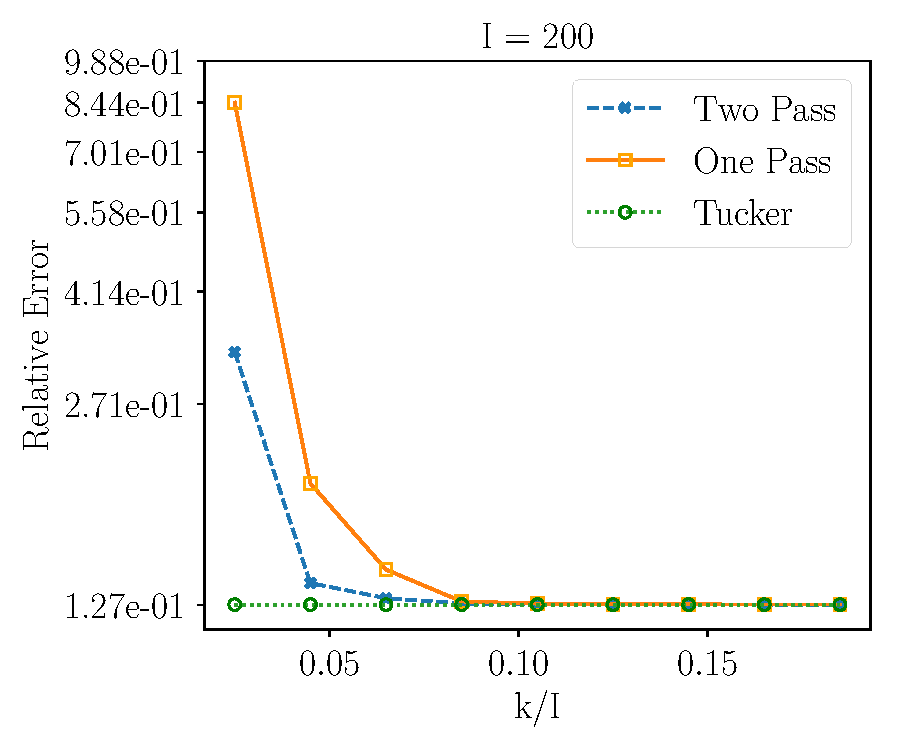
\includegraphics[scale = 0.3]{figure/fpd_n200.pdf}
    \end{subfigure}
    \begin{subfigure}{0.32\textwidth}
    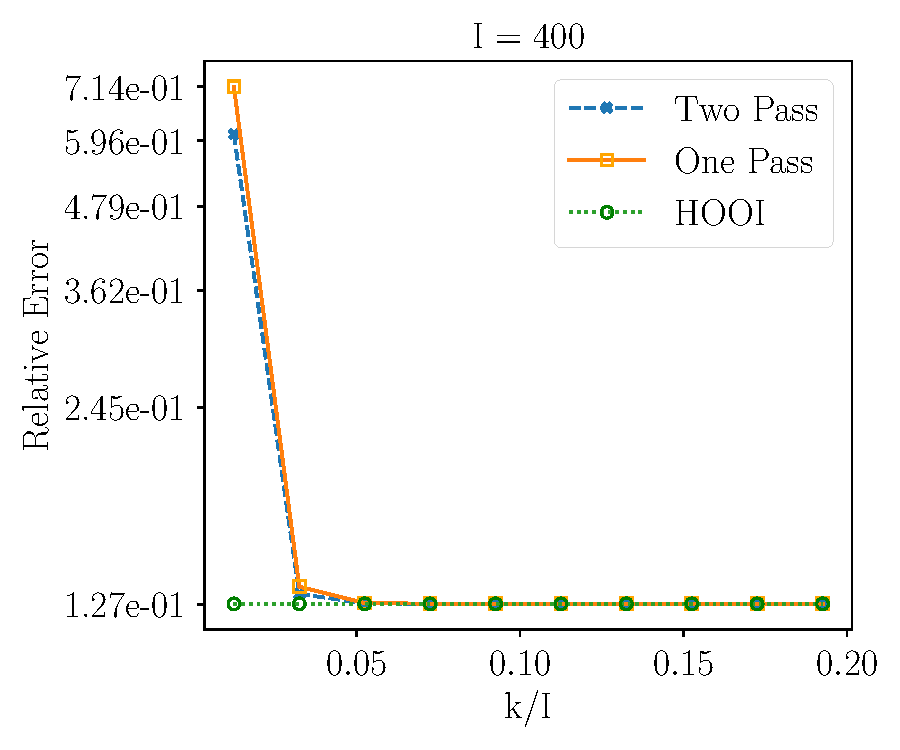
\includegraphics[scale = 0.3]{figure/fpd_n400.pdf}
    \end{subfigure}
    \begin{subfigure}{0.32\textwidth}
    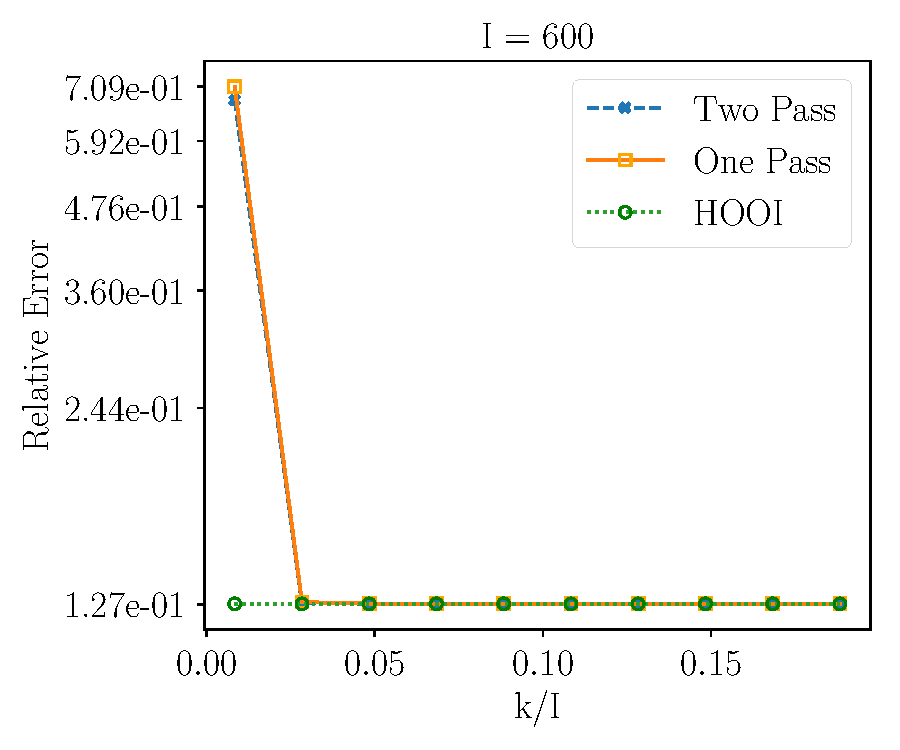
\includegraphics[scale = 0.3]{figure/fpd_n600.pdf}
    \end{subfigure}
\textbf{Superdiagonal + Low Noise ($\gamma = 0.01, \, r = 1$)}\\
    \centering 
    \begin{subfigure}{0.32\textwidth}
    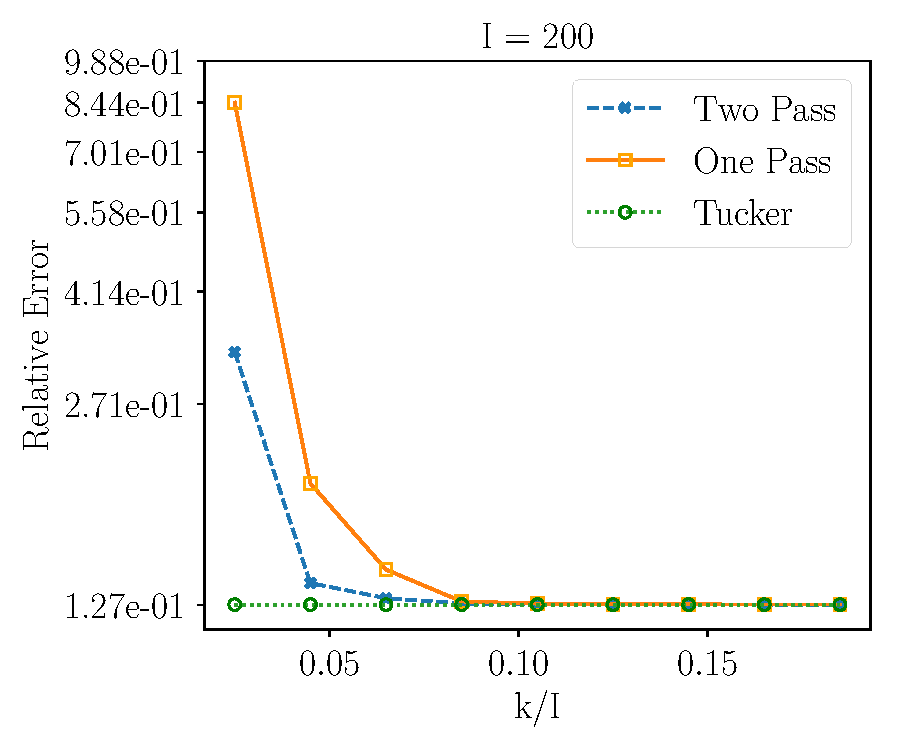
\includegraphics[scale = 0.3]{figure/fpd_n200.pdf}
    \end{subfigure}
    \begin{subfigure}{0.32\textwidth}
    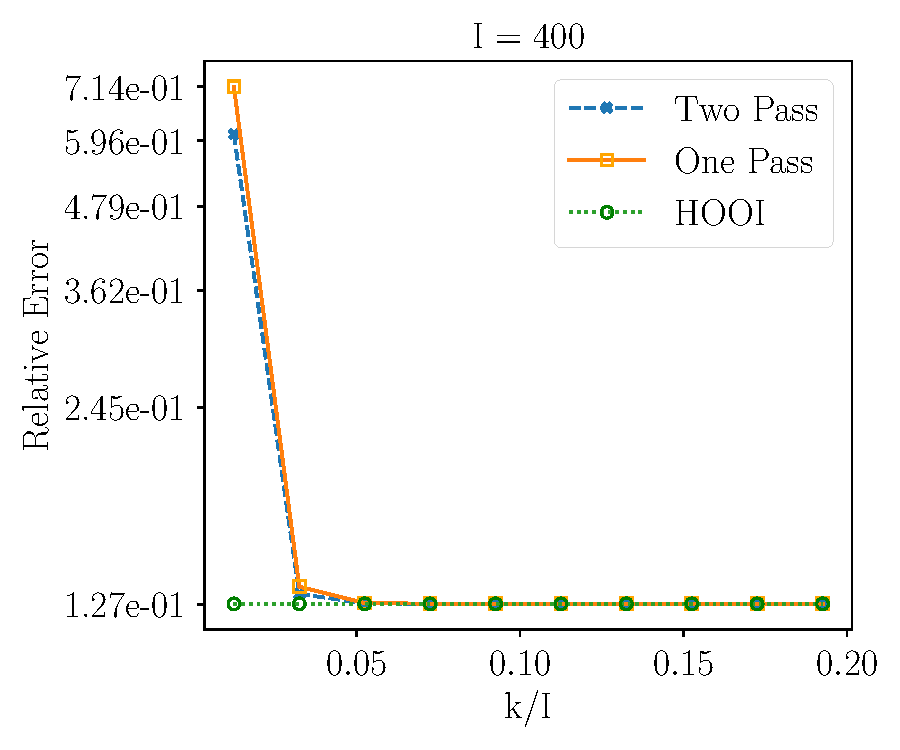
\includegraphics[scale = 0.3]{figure/fpd_n400.pdf}
    \end{subfigure}
    \begin{subfigure}{0.32\textwidth}
    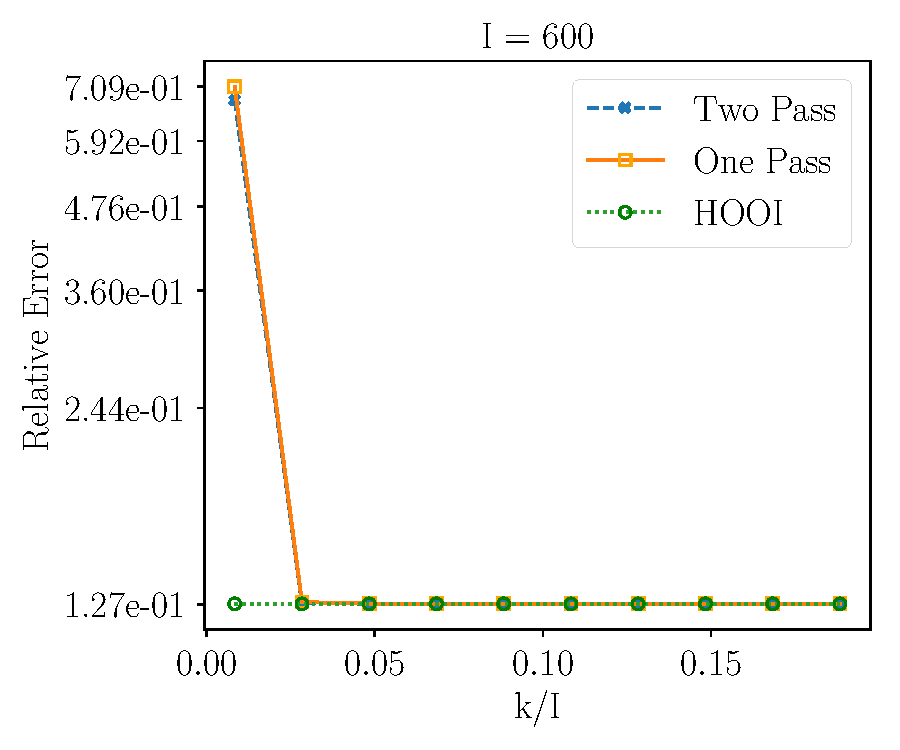
\includegraphics[scale = 0.3]{figure/fpd_n600.pdf}
    \end{subfigure}
\textbf{Fast Polynomial Decay ($t = 2$)}\\
    \centering 
    \begin{subfigure}{0.32\textwidth}
    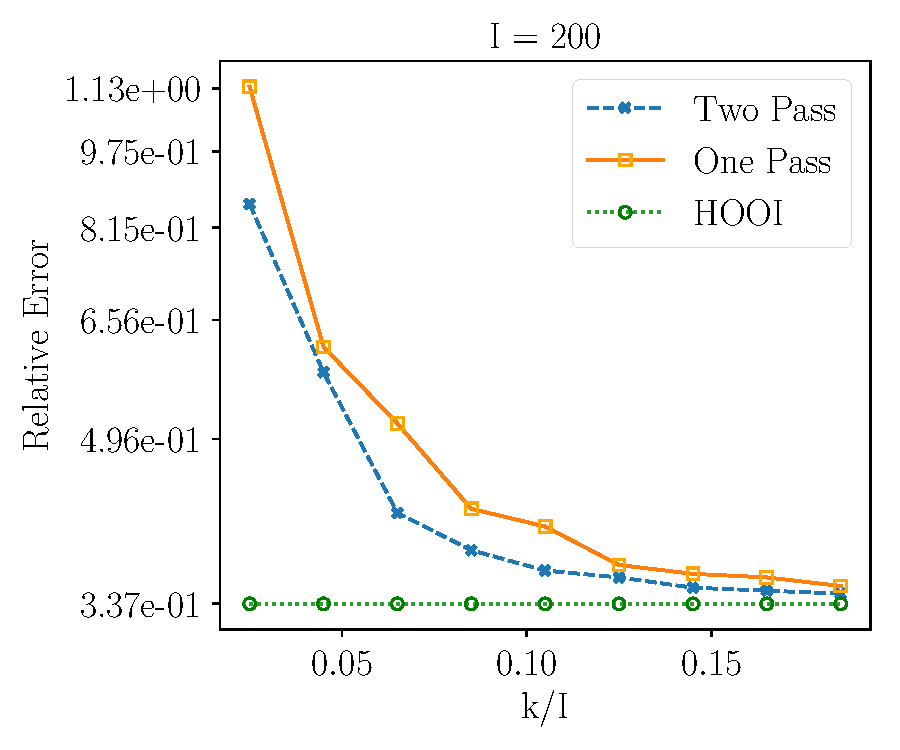
\includegraphics[scale = 0.3]{figure/spd_n200.pdf}
    \end{subfigure}
    \begin{subfigure}{0.32\textwidth}
    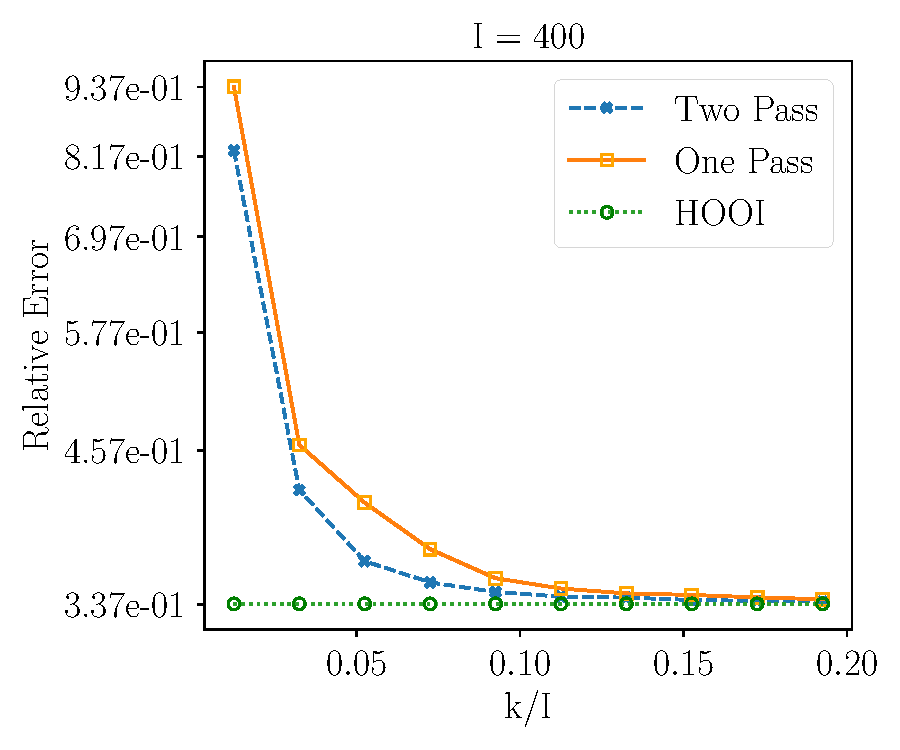
\includegraphics[scale = 0.3]{figure/spd_n400.pdf}
    \end{subfigure}
    \begin{subfigure}{0.32\textwidth}
    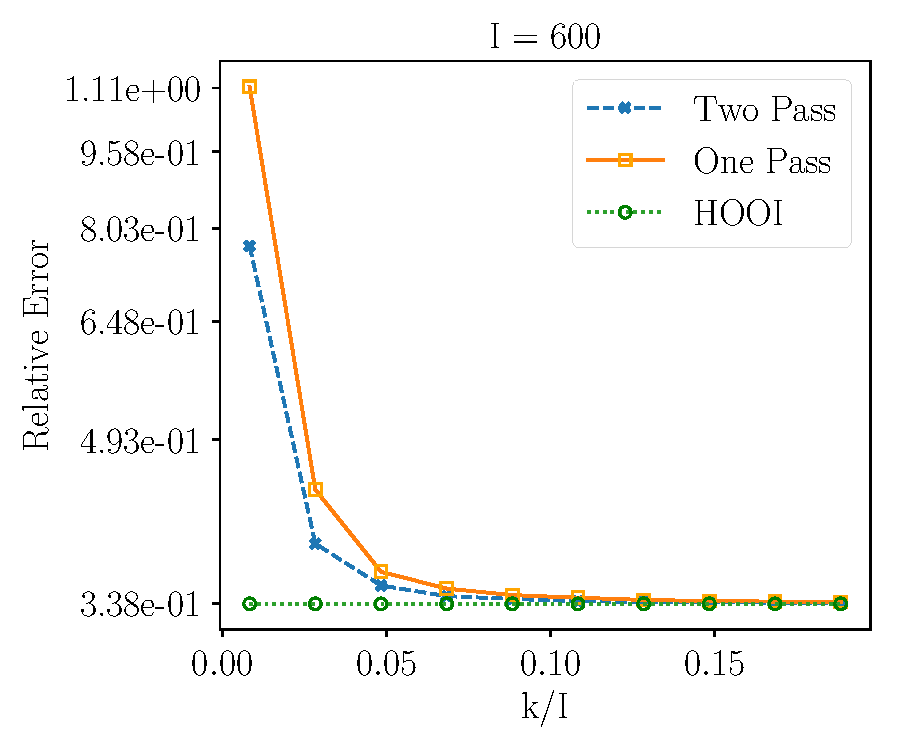
\includegraphics[scale = 0.3]{figure/spd_n600.pdf}
    \end{subfigure}
\textbf{Slow Polynomial Decay ($t = 1$)}\\
    \centering 
    \begin{subfigure}{0.32\textwidth}
    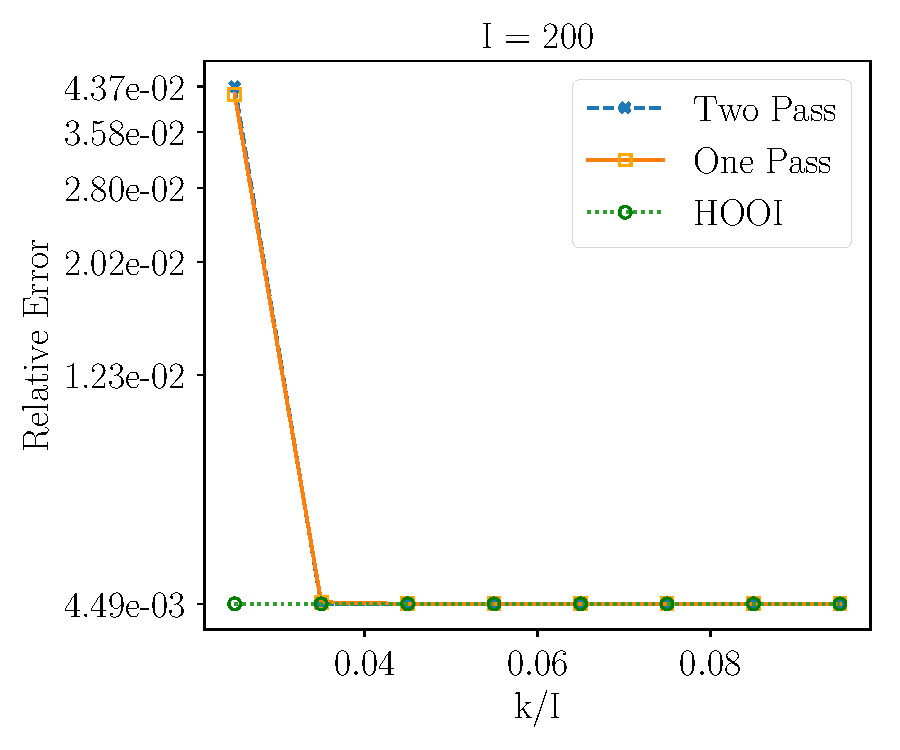
\includegraphics[scale = 0.3]{figure/fed_n200.pdf}
    \end{subfigure}
    \begin{subfigure}{0.32\textwidth}
    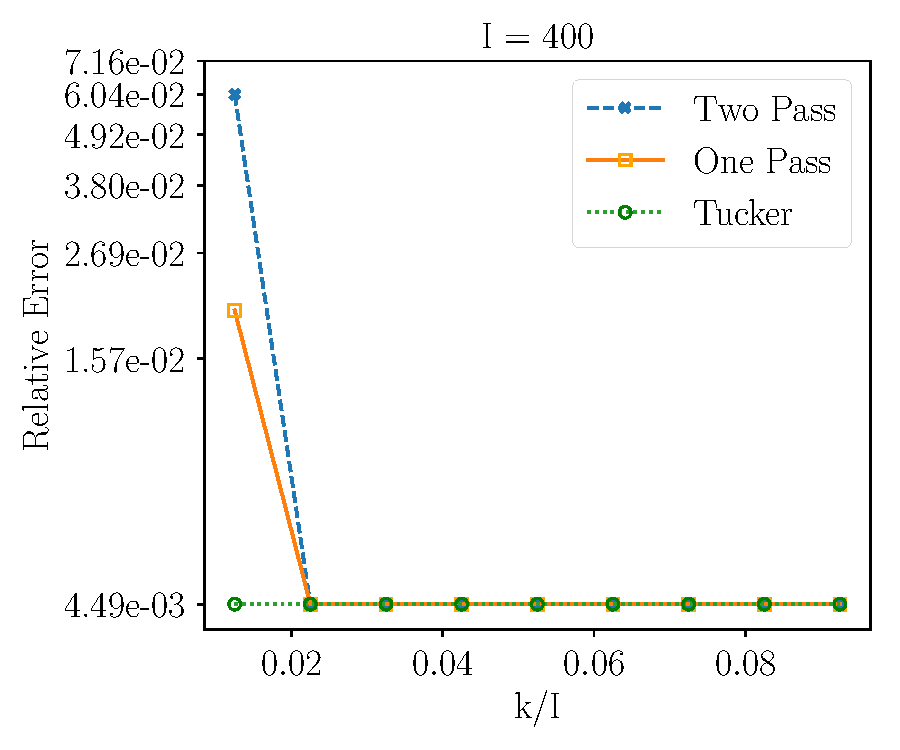
\includegraphics[scale = 0.3]{figure/fed_n400.pdf}
    \end{subfigure}
    \begin{subfigure}{0.32\textwidth}
    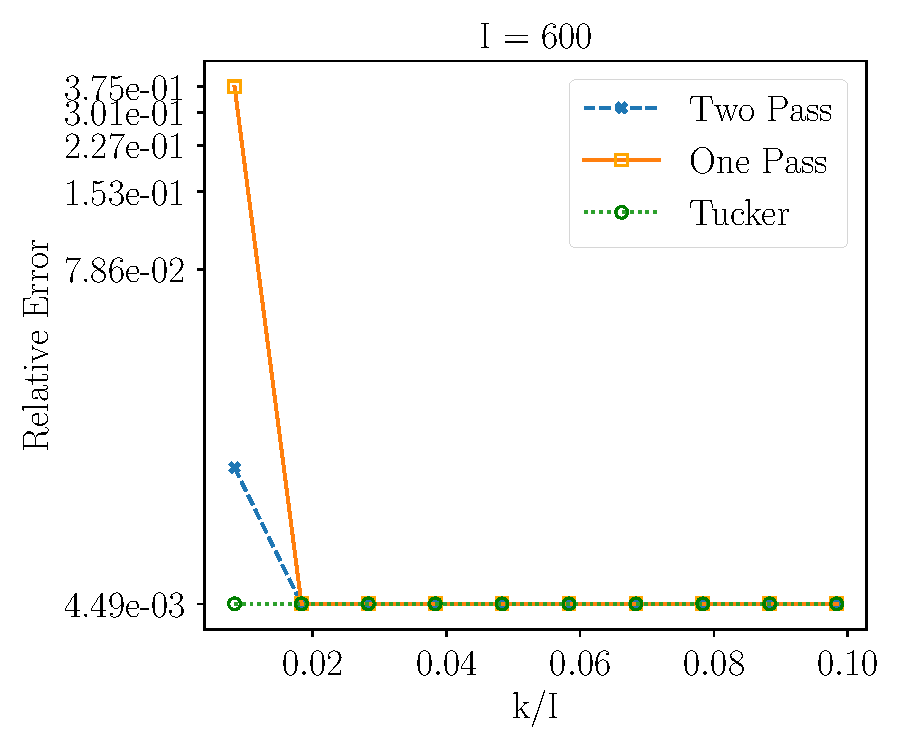
\includegraphics[scale = 0.3]{figure/fed_n600.pdf}
    \end{subfigure}
\textbf{Fast Exponential Decay ($t = 1$)}\\
    \centering 
    \begin{subfigure}{0.32\textwidth}
    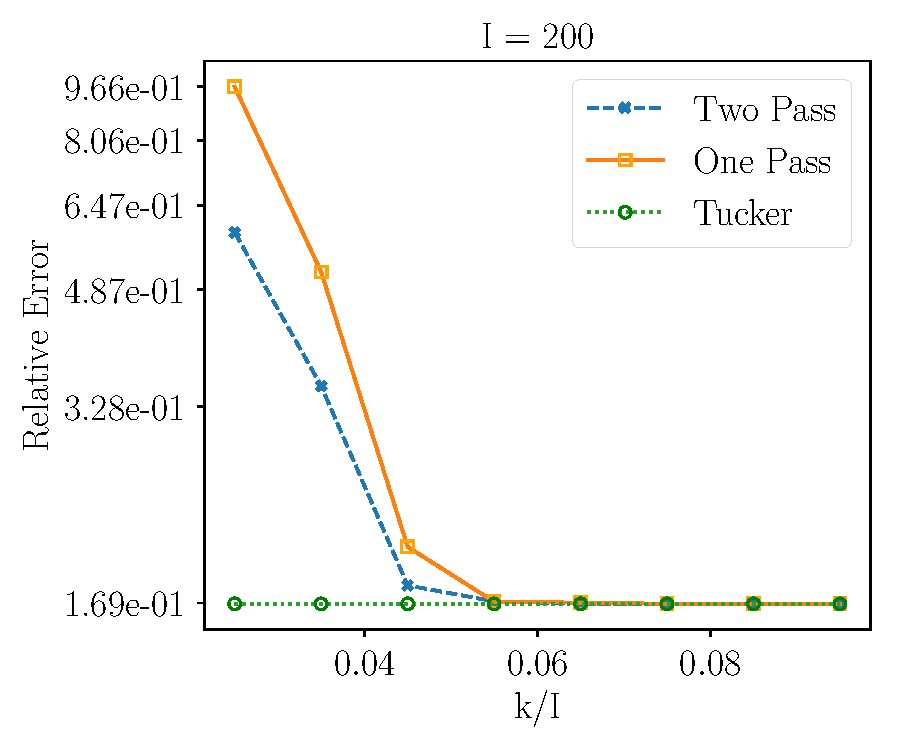
\includegraphics[scale = 0.3]{figure/sed_n200.pdf}
    \end{subfigure}
    \begin{subfigure}{0.32\textwidth}
    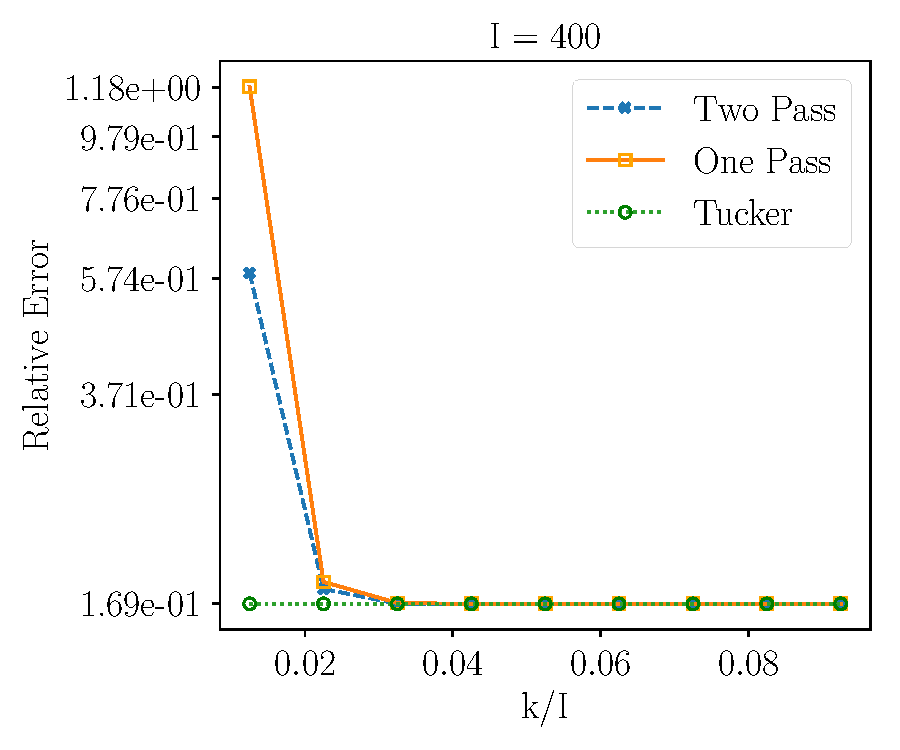
\includegraphics[scale = 0.3]{figure/sed_n400.pdf}
    \end{subfigure}
    \begin{subfigure}{0.32\textwidth}
    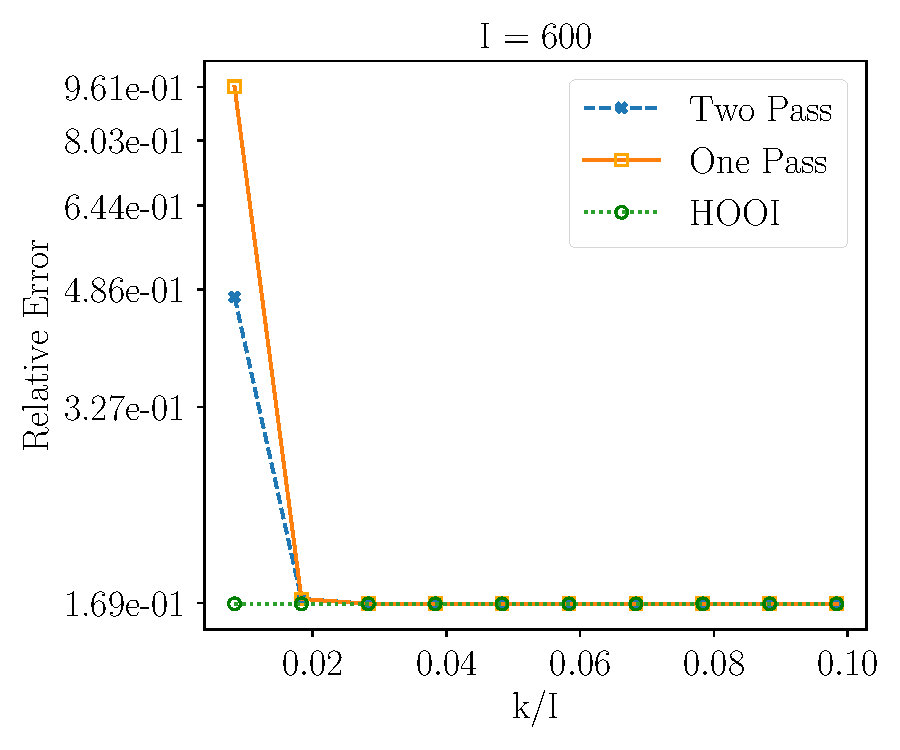
\includegraphics[scale = 0.3]{figure/sed_n600.pdf}
    \end{subfigure}
\textbf{Slow Exponential Decay ($t = 0.25$)} \\ 
\captionsetup{labelformat=empty}
\end{figure}

\setcounter{figure}{2}    
\begin{figure}[H]
\centering
    \begin{subfigure}{0.32\textwidth}
    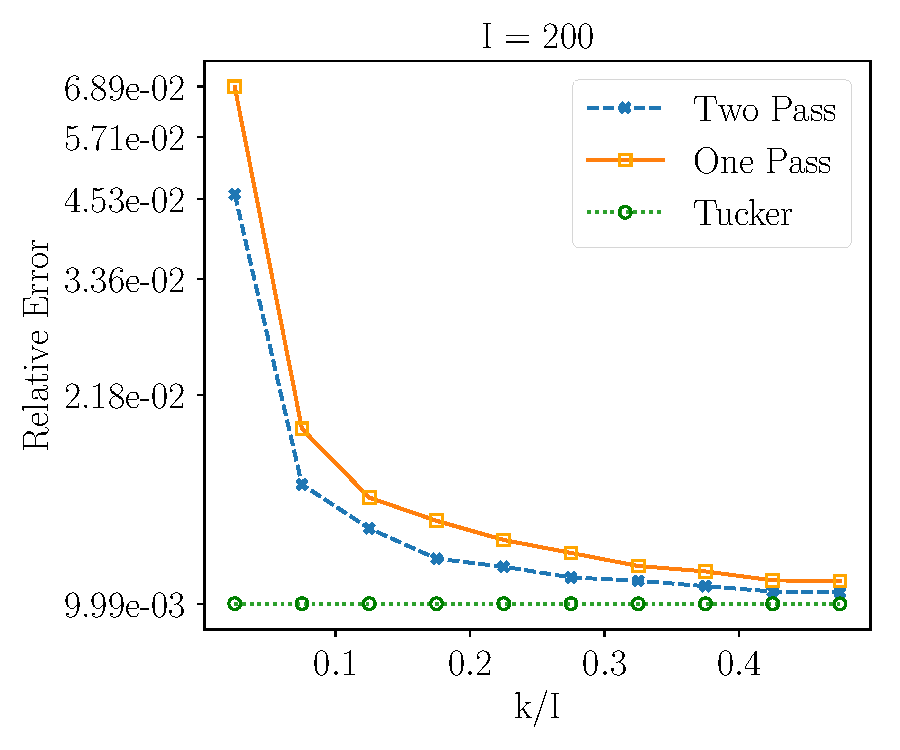
\includegraphics[scale = 0.3]{figure/lk_lnoise_n200.pdf}
    \end{subfigure}
    \begin{subfigure}{0.32\textwidth}
    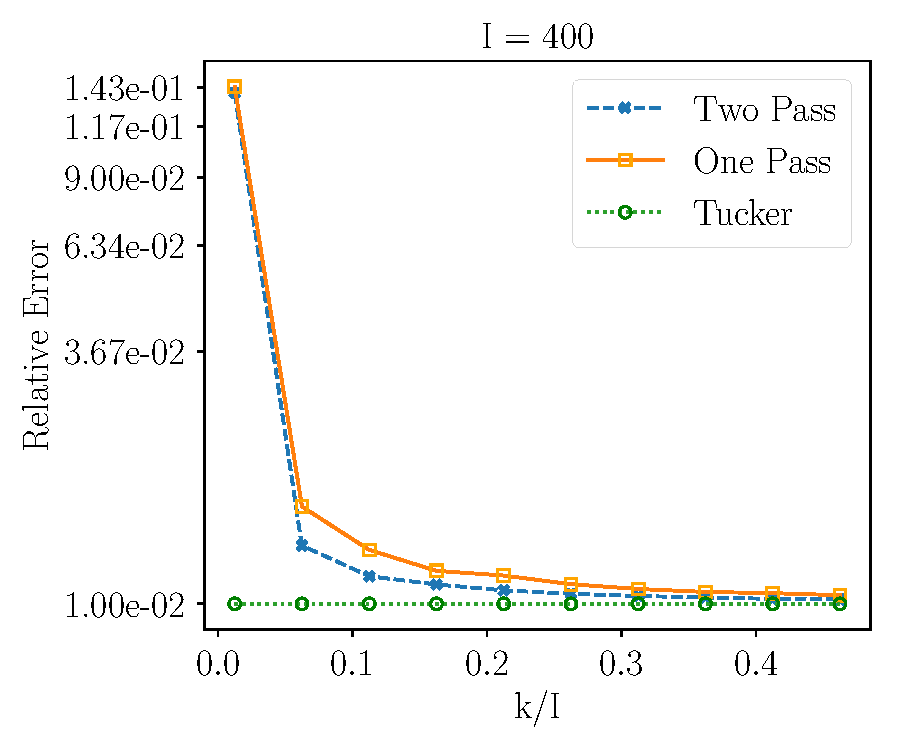
\includegraphics[scale = 0.3]{figure/lk_lnoise_n400.pdf}
    \end{subfigure}
    \begin{subfigure}{0.32\textwidth}
    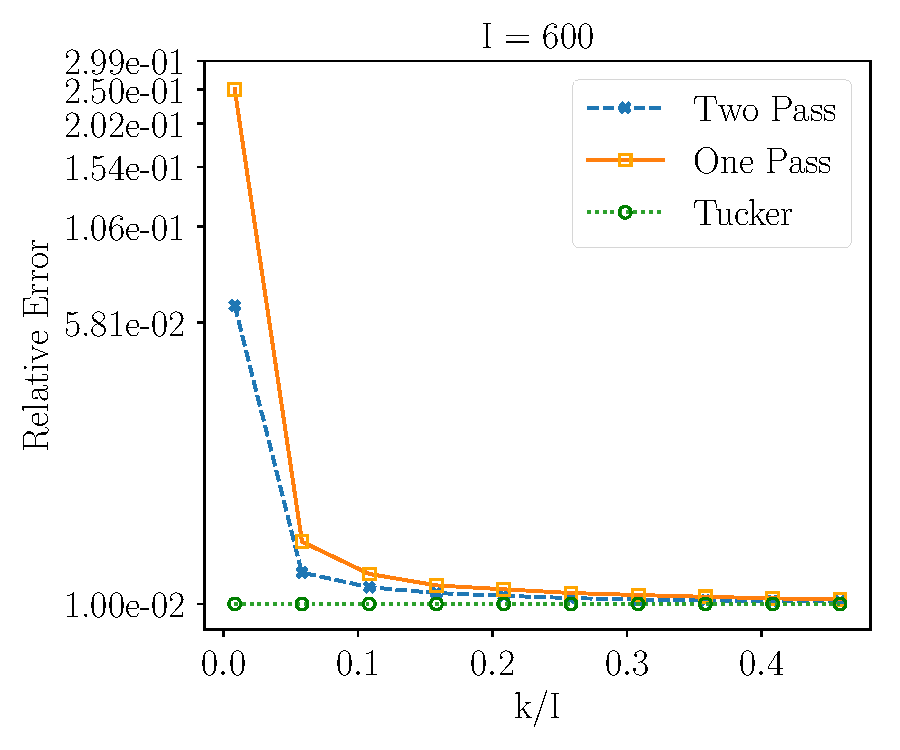
\includegraphics[scale = 0.3]{figure/lk_lnoise_n600.pdf}
    \end{subfigure}
\textbf{Low Rank + Low Noise ($\gamma = 0.01$)} \\ 
\centering
    \begin{subfigure}{0.32\textwidth}
    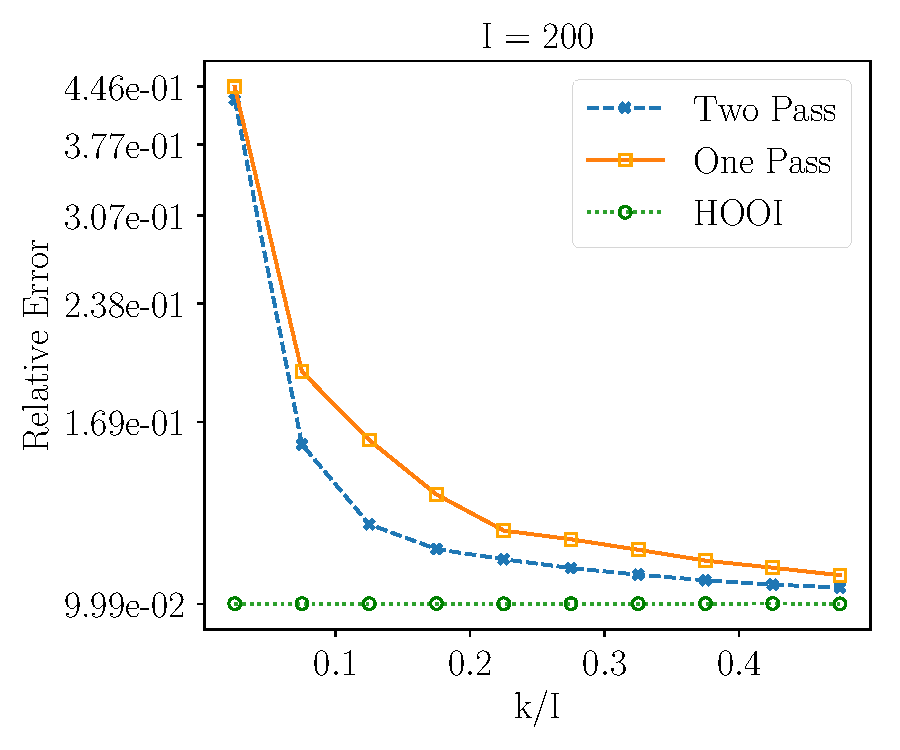
\includegraphics[scale = 0.3]{figure/lk_mnoise_n200.pdf}
    \end{subfigure}
    \begin{subfigure}{0.32\textwidth}
    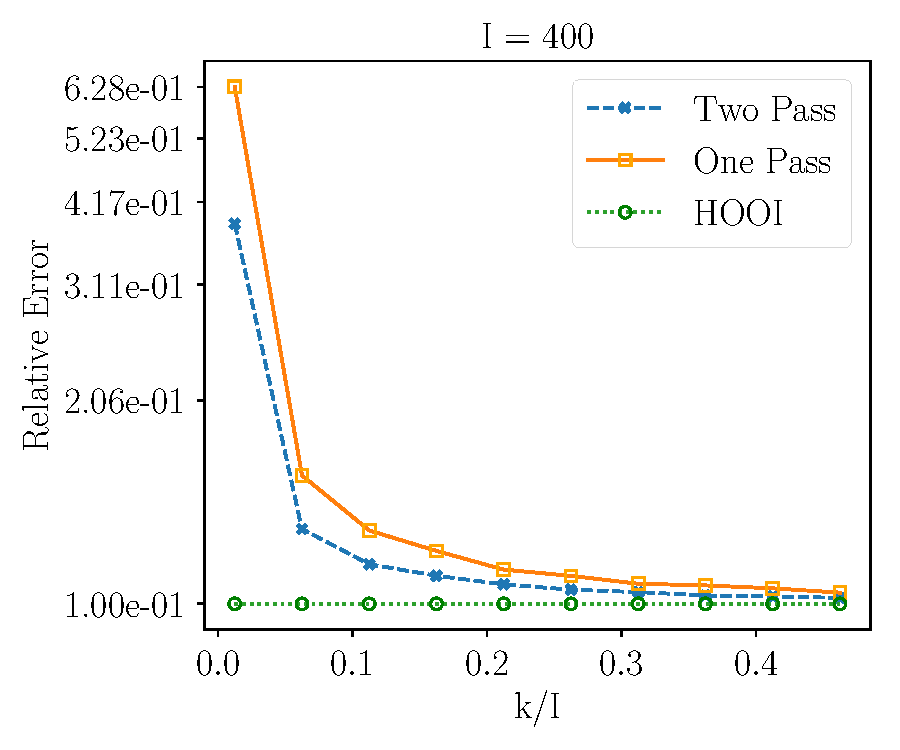
\includegraphics[scale = 0.3]{figure/lk_mnoise_n400.pdf}
    \end{subfigure}
    \begin{subfigure}{0.32\textwidth}
    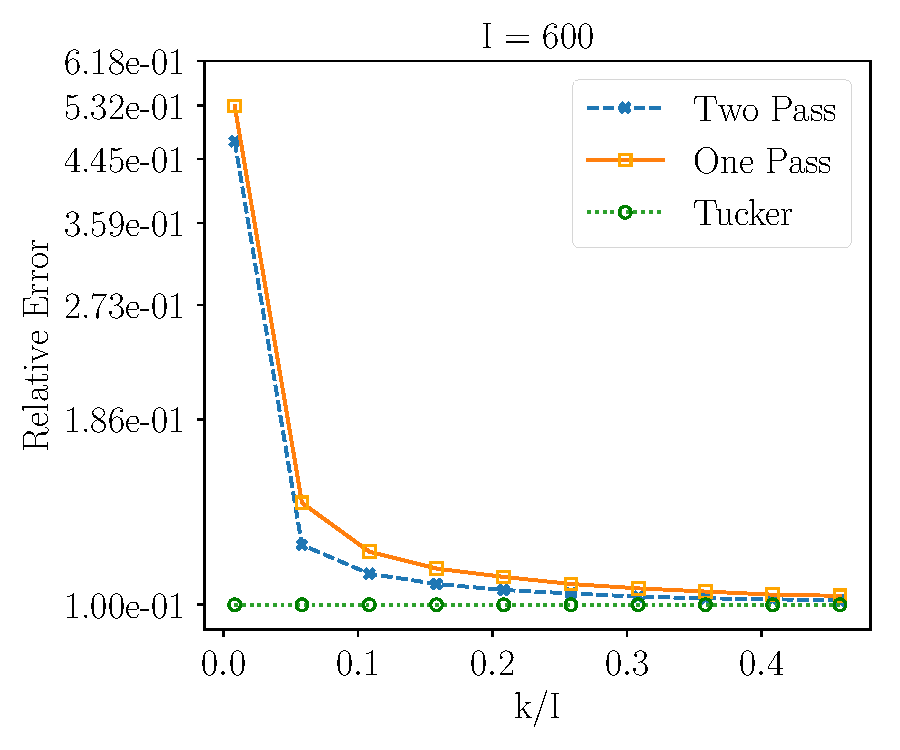
\includegraphics[scale = 0.3]{figure/lk_mnoise_n600.pdf}
    \end{subfigure}
\textbf{Low Rank + Medium Noise ($\gamma = 0.1$)} \\ 
    \begin{subfigure}{0.32\textwidth}
    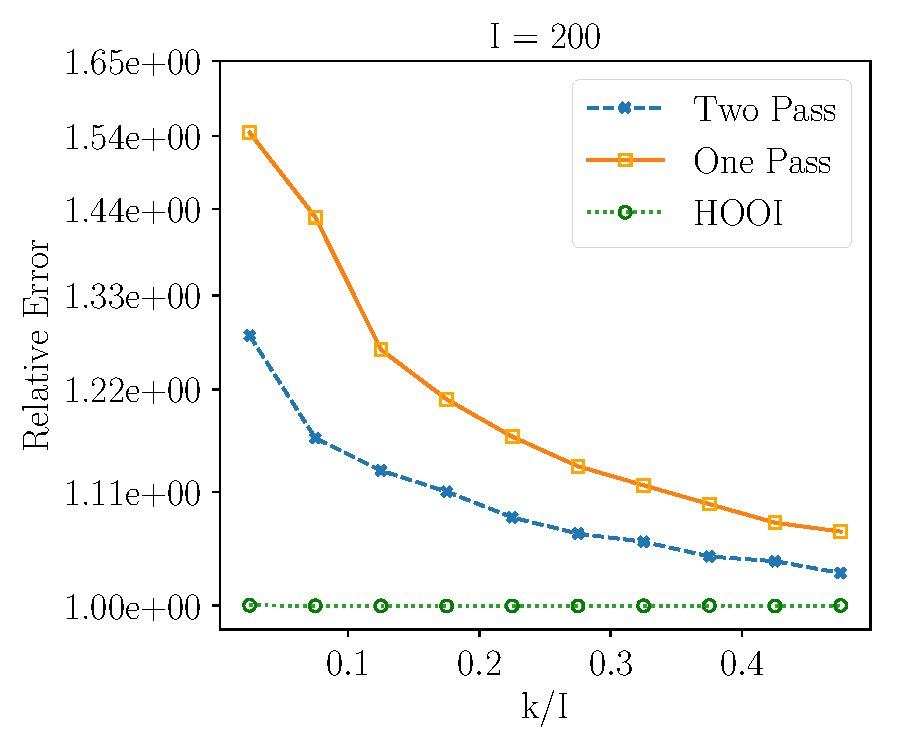
\includegraphics[scale = 0.3]{figure/lk_hnoise_n200.pdf}
    \end{subfigure}
    \begin{subfigure}{0.32\textwidth}
    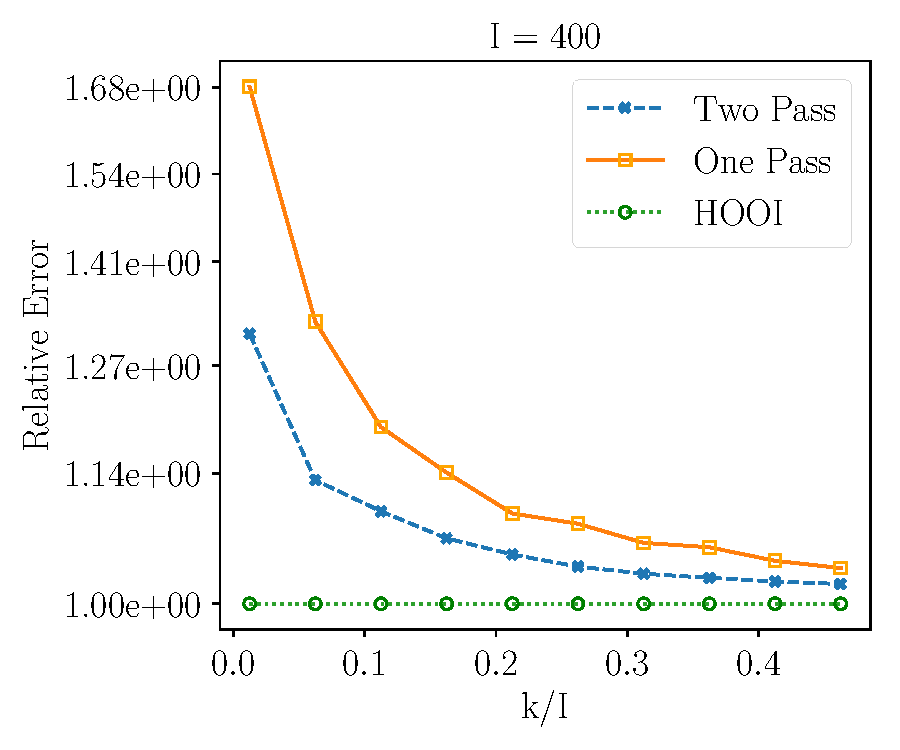
\includegraphics[scale = 0.3]{figure/lk_hnoise_n400.pdf}
    \end{subfigure}
    \begin{subfigure}{0.32\textwidth}
    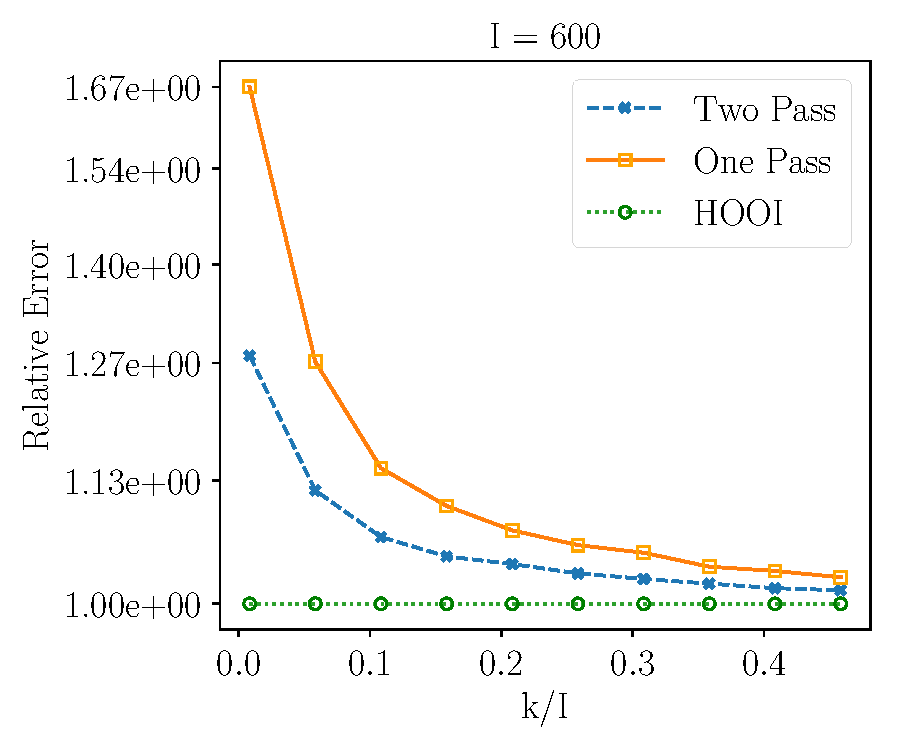
\includegraphics[scale = 0.3]{figure/lk_hnoise_n600.pdf}
    \end{subfigure}
\textbf{Low Rank + High Noise ($\gamma = 1$)} \\ 

\caption{Relative error for fixed-rank tensor approximation as a function of the compression factor $k/n$: \textit{We compare the relative error presented in log scale for two-pass sketching, one-pass sketching and Tucker decomposition for different design tensors when n = 200, 400, 600. $r = 5$ except for the first row.}} \label{fig:more_result}
\end{figure}


\section{More Real Data Results}\label{appendix: more_real_data_result}
\begin{figure}[H]
    \centering
    \begin{subfigure}{0.32\textwidth}
    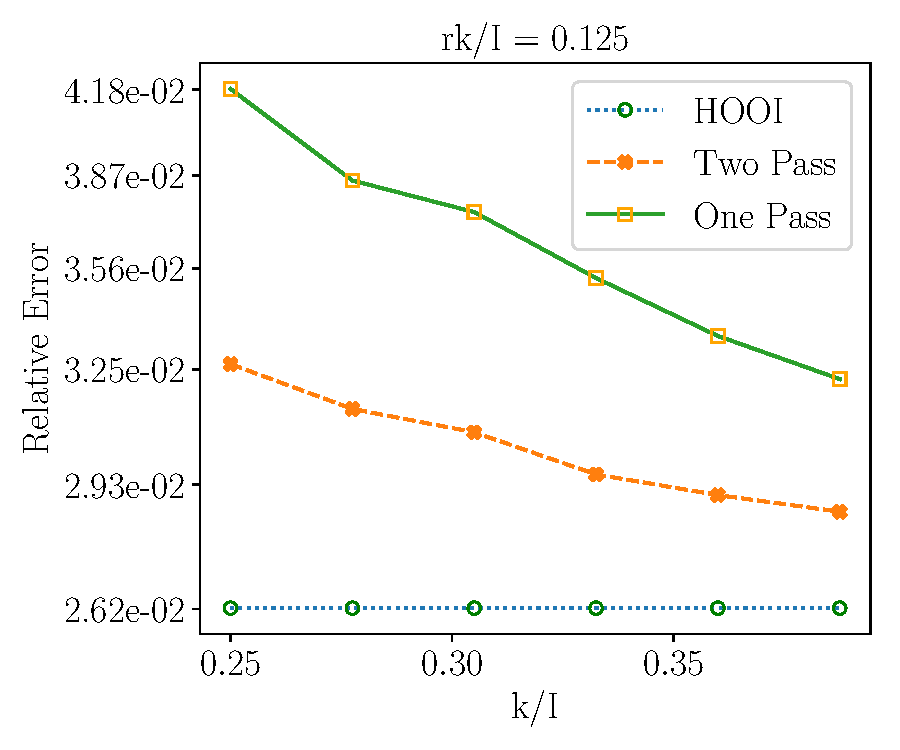
\includegraphics[scale = 0.3]{figure/SRFRAD_frk8.pdf}
    \end{subfigure}
    \begin{subfigure}{0.32\textwidth}
    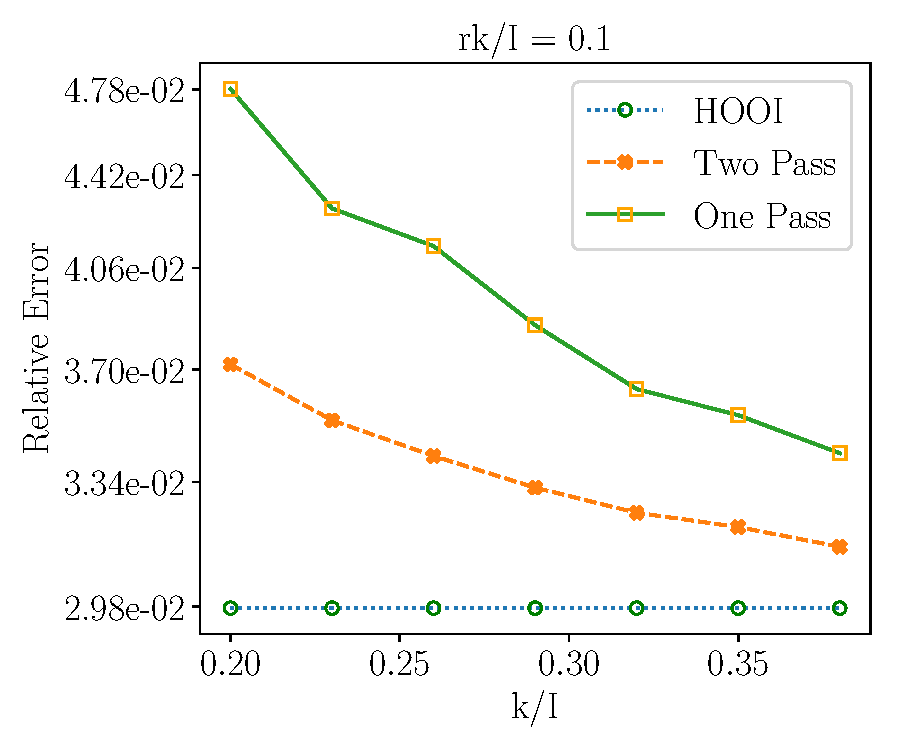
\includegraphics[scale = 0.3]{figure/SRFRAD_frk10.pdf}
    \end{subfigure}
    \begin{subfigure}{0.32\textwidth}
    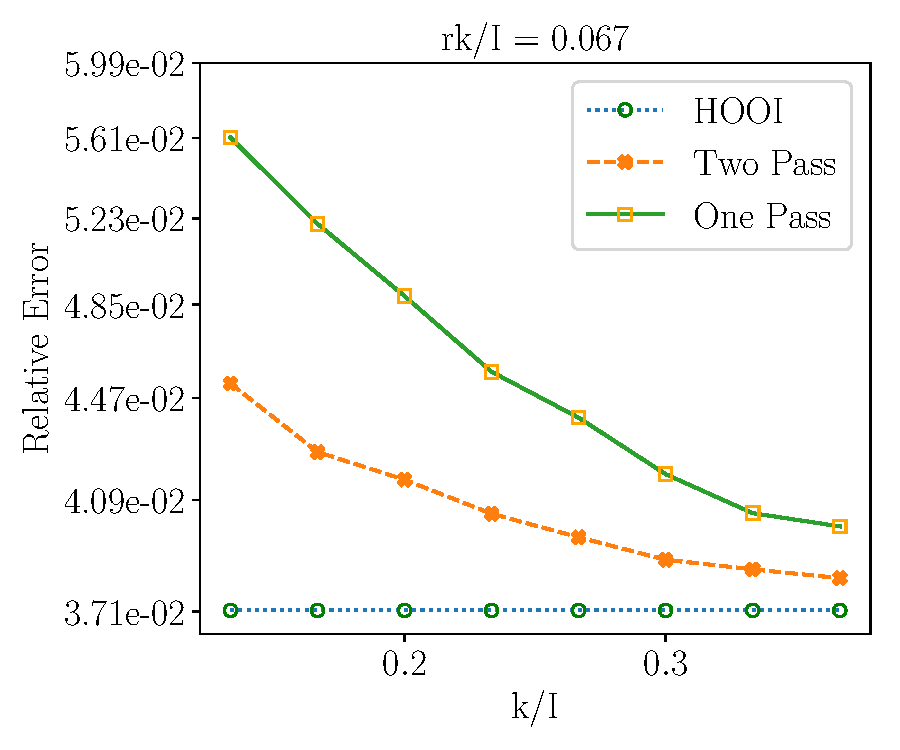
\includegraphics[scale = 0.3]{figure/SRFRAD_frk15.pdf}
    \end{subfigure}\\ 
    \textbf{Net Radiative Flux at Surface}
    \caption{Relative error for fixed-rank tensor approximation on the net radiative flux data ($1200 \times 192 \times 288$): \textit{We compare the relative errors presented in log scale for two-pass sketching, one-pass sketching and Tucker decomposition with different ranks ($rk/I = 0.125,0.2,0.067$). The dataset comes from the CESM CAM and the net radiative flux determines the energy received by the earth surface through radiation}} \label{fig:srfrad}
\end{figure}
\begin{figure}
    \centering
    \begin{subfigure}{0.32\textwidth}
    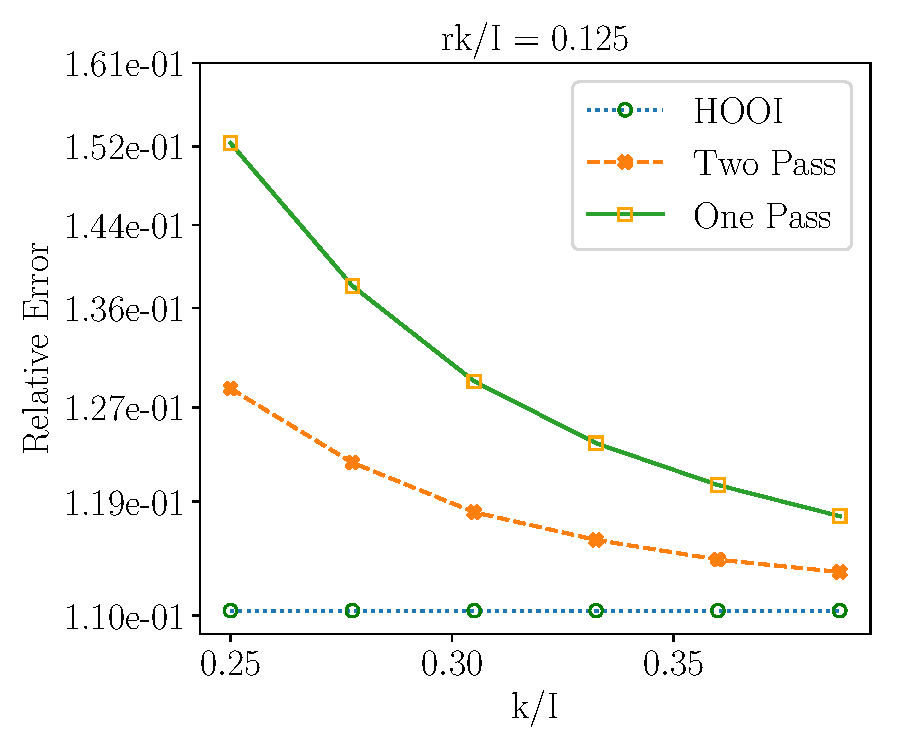
\includegraphics[scale = 0.3]{figure/BURDENDUST_frk8.pdf}
    \end{subfigure}
    \begin{subfigure}{0.32\textwidth}
    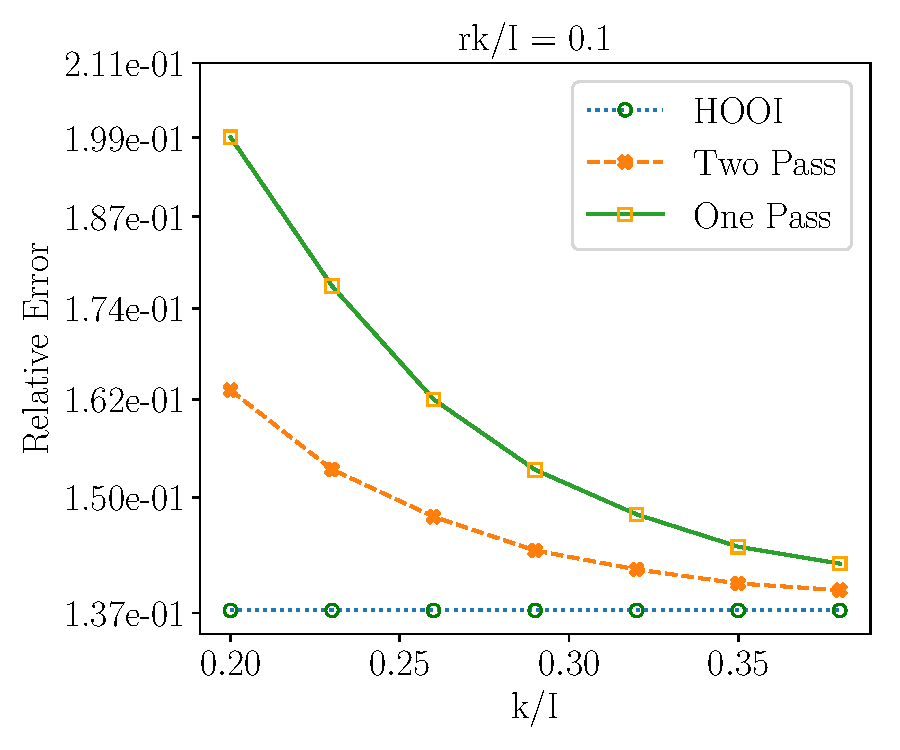
\includegraphics[scale = 0.3]{figure/BURDENDUST_frk10.pdf}
    \end{subfigure}
    \begin{subfigure}{0.32\textwidth}
    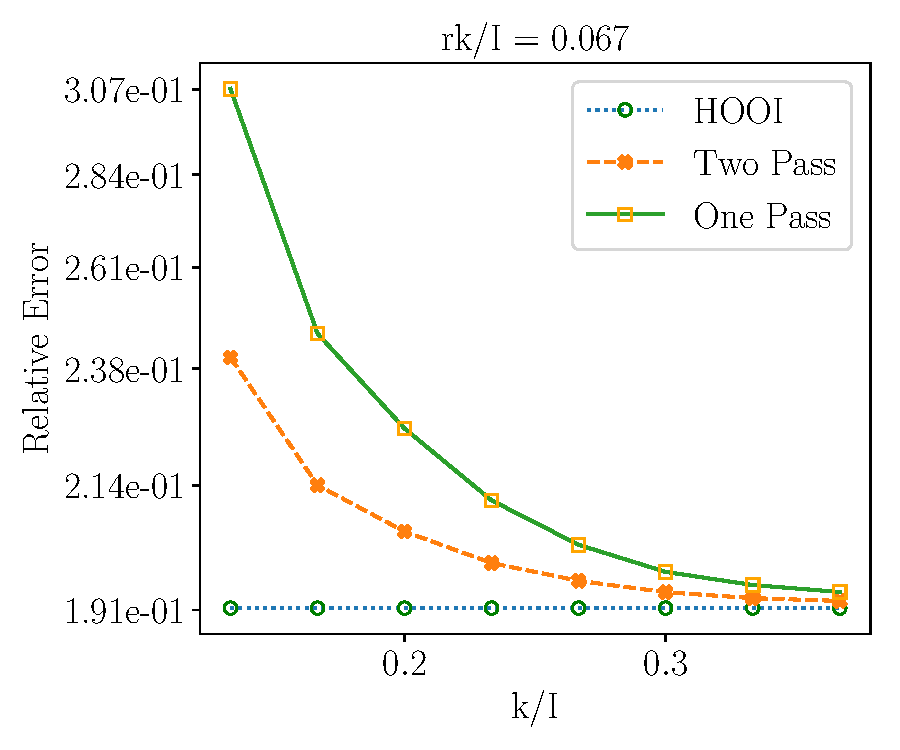
\includegraphics[scale = 0.3]{figure/BURDENDUST_frk15.pdf}
    \end{subfigure}
    \textbf{Dust Aerosol Burden}
    \caption{Relative error for fixed-rank tensor approximation on the dust aerosol burden data ($1200 \times 192 \times 288$): \textit{We compare the relative errors presented in log scale for two-pass sketching, one-pass sketching and Tucker decomposition with different ranks ($rk/I = 0.125,0.2,0.067$). The dataset comes from the CESM CAM and the dust aerosol burden measures the amount of aerosol contributed by the dust.}} \label{fig:burden_dust}
\end{figure}
\section{Computational Complexity} \label{appendix: time-complexity}

\paragraph{Flops for Batch}
In the sketching stage of the two-pass algorithms, we need to first compute the arm sketches, $\mathbf{G}_n = \mathbf{X}\mathbf{\Omega}_n, n \in [N]$ with $kN\hat{I}$ flops in total. Then, in the recovery stage, we first perform "economy size" QR factorizations on $\mathbf{G}_1, \dots, \mathbf{G}_N$ with $\mathscr{O}(k^2(\sum_{n =1}^N I_n))$ to find the orthonormal bases $\mathbf{Q}_1, \dots, \mathbf{Q}_N$. Then, we compute the linkage tensor $\mathscr{W}$ by recursively multiplying $\mathscr{X}$ by $\mathbf{Q}_n^\top, n \in [N]$, with $(k\cdot I_1 \cdot I_{(-1)} + k \cdot I_2 \cdot \frac{I_{(-2)}\cdot k}{I_1} + \cdots + k^{N}\cdot I_N)$ flops, which is bounded by $\mathcal{O}(\frac{k(1-\delta_1^N)\bar{I}}{1-\delta_1})$. The multiplication step together with the arm sketch computation dominates the total cost as in Table \ref{tbl: time-complexity}. 

In the sketching case, the one-pass algorithm needs to additionally compute the core tensor sketch $\mathscr{Z}$ by recursively multiplying $\mathscr{X}$ by $\mathbf{\Phi}_n, n \in [N]$. We can find the upper bound for the number of flops to be $\frac{s(1-\delta_1^N)}{1-\delta_1}\bar{I}$. Finding the orthonormal basis of the arm sketch takes $\mathscr{O}(k^2(\sum_{n =1}^N I_n))$ similar to the two-pass algorithm. To find the linkage tensor $\mathscr{W}$, we need to recursively solve linear square problems, with $\frac{k^2s^N(1-(k/s)^N)}{1-k/s}$ flops. The sketch computation dominates the total time complexity, which is higher than the total time cost of the two-pass algorithm with a different compression factor.

The higher order SVD directly acts on $\mathscr{X}$ by first computing the SVD for each unfolding in $\mathscr{O}(kN\bar{I})$, and then multiplying $\mathscr{X}$ by $\mathbf{U}_1^\top, \dots, \mathbf{U}_N^\top$ in $\mathcal{O}(\frac{k(1-\delta_1^N)\bar{I}}{1-\delta_1})$. The total time cost is approximately the same as the two-pass algorithm. Note: we can use the randomized SVD in the first step to improve the computational cost to $\bar{I}N\log k + \sum_{n = 1}^N(I_{n}+I_{(-n)})k^2$ \cite{halko2011finding}. 

\paragraph{Flops for Streaming} Using the elementwise representation of the mode product, we can significantly simplify the computation for sparse input tensor in the streaming model. In computing the arm sketches for both one-pass and two-pass algorithm, the complexity goes from $kN\bar{I}$ to $\mu kN\bar{I}$. Furthermore, we can reduce the computational complexity of multiplying $\mathscr{X}$ by $\mathbf{Q}_1^T, \dots, \mathbf{Q}_N^T$ from $\mathscr{O}(\frac{k(1-\delta_1^N)\bar{I}}{1-\delta_1})$ to $\mathscr{O}(\mu k^N N(\sum_{n =1}^N I_n ))$ in the recovery stage of the two-pass algorithm. Similarly, we can reduce the complexity of multiplying $\mathscr{X}$ by $\mathbf{\Phi}_1, \dots, \mathbf{\Phi}_N$ from $\frac{s(1-\delta_2^N)\bar{I}}{1-\delta_2}$ to $\mu s^NN(\sum_{n=1}^NI_n)$ in the sketching phase of one-pass algorithm. The higher order SVD, in comparison, does not support the streaming model. 

\section{Review of Tensor Algorithmic Operators}
\label{sec:review_tensor}
We review some basic tensor algorithmic operators first. Let $\mathscr{X}$ be the tensor of shape $I_1\times I_2\times \dots \times I_N$. For tensor product with distinct modes ($m\neq n$), the order of mode products does not matter:
\begin{equation}
\label{eq: tensor_product_mul_exchangable}
\mathscr{X}\times_m \mathbf{A} \times_n \mathbf{B} =    \mathscr{X}\times_n \mathbf{B} \times_m \mathbf{A}. 
\end{equation}
If the modes are the same, then 
\begin{equation}
\label{eq: tensor_product_association}
\mathscr{X}\times_n \mathbf{A} \times_n \mathbf{B} =    \mathscr{X}\times_n (\mathbf{BA}). \end{equation}
It is worth noting that the inner product for tensors is the same with respect to any mode-n matricization, with its definition given by
\begin{equation}
\label{eq:F_norm_equivalent}
\langle \mathscr{X}, \mathscr{Y}\rangle = \langle \mathbf{X}^{n}, \mathbf{Y}^{(n)}\rangle = \rm{Tr}((\mathbf{X}^{(n)})^\top \mathbf{Y}^{(n)}). 
\end{equation}
\end{appendices}
 



\end{document}